%-*-    coding: UTF-8   -*-
\documentclass[UTF-8]{ctexart}

\usepackage{graphicx}
\usepackage{subfigure}
\usepackage{amsmath}
\usepackage{geometry}%页面设置
\usepackage{tabularx}%表格扩展
\usepackage{color}
\usepackage{xcolor}
\usepackage{hyperref}
\usepackage{ulem}
\usepackage{multirow}%表格合并
\usepackage{amsmath}%数学公式
\usepackage{longtable}%表格跨页
\usepackage[cache=false]{minted}%代码高亮
\usepackage{fontspec,xunicode,xltxtra}
\usepackage{fontspec}%字体设置
%取消链接的红框
\hypersetup{
	colorlinks=true,
	linkcolor=black
}

%A4纸大小,版心居中,长宽占页面的0.8
\geometry{a4paper,centering,scale=0.8}
%改变图表标题格式,此处使用悬挂对齐方式(编号向左突出),小字号,标题使用斜体
\usepackage[format=hang,font=small,textfont=it]{caption}
%增加目录项目,tocbibind宏包会自动加入目录项本身、参考文献、索引等项目。[nottoc]取消了对自身的显示
\usepackage[nottoc]{tocbibind}

%定义代码高亮,方便下面编写
\definecolor{bg}{rgb}{0.95,0.95,0.95}
\newcommand{\cpp}[1]{\inputminted[bgcolor=bg,breaklines,breakanywhere=true]{c++}{#1}}

%字体声明,等宽字体采用 Ubuntu Mono
\setmonofont{Ubuntu Mono}

%title 信息
\title{OI 复习资料}
\author{SYCstudio}
\date{\today}

\begin{document}
	\maketitle%输出题目
	\newpage
	\tableofcontents%输出目录
	\newpage%换页
	%\section{前言}
	\section{基本操作}
		\subsection{高精度相关}
			\subsubsection{高精度整数}
			\cpp{code//Basic//biginteger.cpp}
			\subsubsection{高精度分数}
			\cpp{code//Basic//bigfraction.cpp}
		\subsection{输入输出优化}
		\cpp{code//Basic//io.cpp}
		\subsection{实用卡常技巧}
			\subsubsection{手写 $gcd$}
			原理是更相减损术。
			\cpp{code//Basic//fastgcd.cpp}
			\subsubsection{强制展开}
			也不知道有什么用。不推荐使用。

			\mintinline{c++}{__attribute__((always_inline))}
	\newpage
	\section{基础算法}
		\subsection{搜索}
		基于 $dfs$ 或者 $bfs$ 的全解枚举算法。
			\subsubsection{常见优化}
			\begin{itemize}
				\item 剪枝:可行性剪枝,最优化剪枝。
				\item 迭代加深搜索:结合两家之长。
				\item 启发式搜索:$A$ 和 $IDA$。
				\item 记忆化搜索:有效避免子问题的重复计算。
			\end{itemize}
			\subsubsection{整数的拆分方案}
			如果是求方案数,有比较简单的动态规划方法,而对于方案的求法,一般采用搜索。通常用来预处理合法方案以减少复杂度。
			\subsubsection{打表与结论}
			可以用搜索来打表猜测结论。
		\subsection{贪心}
		常见与各种优化与思维中。
			\subsubsection{常见模型}
			\begin{itemize}
				\item 序列排序,贪心按左端点或右端点选择。
				\item 田忌赛马。
				\item 绝对值最值问题,选取中位数。
				\item 堆模拟网络流,贪心地模拟退流和补流。
				\item $DP$ 优化,运用贪心排除掉一定不可能成为解的决策,缩小决策范围。
				\item 树上最优化问题考虑直径和重心。
				\item 图上最优化问题考虑生成树和路径树/路径 $DAG$。
				\item 贪心不等式。
				\item 最优化字典序问题,考虑从小到大加入是否会使答案变差。
			\end{itemize}
		\subsection{二分}
		转求解型问题为判定型问题。
			\subsubsection{最值二分}
			求解最值或者边界合法值的问题,如果具有可二分性,即可采用二分转变为判定性问题。
			通常在二分后结合贪心,$DP$ 或者其它数据结构来进行判定。
			\subsubsection{分数规划}
			求解形如 $\frac{\sum A_i}{\sum B_j}$ 的最值问题。
	
			二分答案 $mid$ ,然后移项不等式得到二分边界的移动条件,根据是要求最小还是最大,贪心地求得算式的解。
	
			另一种解法是迭代的 Dinkelbach 方法。简单地来说,二分法中对于二分的答案 $mid$ 只利用其进行求解判定,对于当前算出的解直接丢弃了,而 Dinkelbach 则迭代地利用当前得到的解直接更新解,迭代操作,直到得到的解与当前解相同。
	
			迭代初值选取是任意的。通常根据题目性质选择一个合适的边界值。实践来看,Dinkelbach 比二分在常数上更加优秀一些。
			\subsubsection{带权二分/凸优化}
			主要用来解决形如分段、分组或者选择的次数有限制的情况。对于每一次分割,给分割二分一个权值,这样这个代价越大,分割越少,反之分割越多(当求最小值的时候),这样就可以二分出最后的答案。
	
			这个优化一般可以用来优化掉动态规划的一维,即将一个 $O(n)$ 转化为 $O(\log n)$
	
			本质上是在二分斜率,所以要求答案关于次数的函数是一个凸函数,斜率单调。
	
			看起来需要小数二分,但对于本来全部都是整数的情况,其实整数二分就够用了。当保证有解的时候,可以用一些优先级的处理避免边界判断。
			\subsubsection{三分}
			对于答案关于某个自变量呈单峰函数的,可以采用三分的方式逼近最优值。
	
			当然也可以采用二分斜率的方式达到与三分相同的目的,常数一般更小。
		\subsection{分治}
		分而治之。简单地来说,就是把问题分解文更小的子问题来递归求解,最后合并答案。
			\subsubsection{CDQ 分治}
			先递归左边,然后考虑跨越中间的贡献,或者是用前半部分来计算后半部分,再递归右边。
	
			要求每个修改与询问之间的关系是独立的,也就是说对于某个询问,前面的修改顺序与答案无关。
			\subsubsection{极值分治/启发式分裂}
			每次不再是选择序列的位置中点分治,而是选择极值位置进行分裂。一般用于处理与极值相关的问题,因为这样考虑跨越中间的贡献时,极值是确定的。
	
			为了保证复杂度,一般要求枚举小的一边而用数据结构查询大的一边。
	
			其过程类似倒着进行的按照极值的启发式合并,所以也叫做启发式分裂。
			\subsubsection{线段树分治}
			利用线段树上一个区间最多分成 $O(\log)$ 个节点的优良性质,把询问或者修改下放到线段树上,然后递归整个线段树离线地回答询问。
			\subsubsection{整体二分}
			二分与分治的结合。
	
			考虑二分一次实际上只计算了一个的答案,那么如果对于多个询问,每个询问会得到的不同的回复,把询问按照回复分到当前二分值的左右,递归处理。
	
			注意在处理的时候,单次判断的复杂度只能与当前在该区间的询问的个数线性相关,否则无法保证复杂度。
		\subsection{动态规划}
		一种高效的问题求解方法。一般的关键在于状态的设计和状态的转移。
	
		找出基本模型,然后根据需求添加合适的维度来设计转移。
			\subsubsection{序列动态规划}
			有两种基本形式,一种是枚举当前位置 $i$,维护 $i$ 前面所有的信息 \texttt{F[i]} 。另一种是维护两维表示当前信息的左右端点 \texttt{F[l][r]}  。
			\subsubsection{树上动态规划}
			常见的模型有直接在树上 $DP$ 和按某种顺序转化成序列做 $DP$ 。
	
			注意转移的时候对子树不重不漏的处理。
			\subsubsection{计数概率期望动态规划}
			这几类可以放在一起。本质上难点还是在于如何设计状态和转移,借助数论知识辅助推导方程。
	
			可以借助马尔科夫链得到转移图,设计转移方式。
			\subsubsection{数位动态规划}
			在一般的动态规划基础上加上一维 \texttt{[0/1]} 表示是危险态还是安全态。按位从高到低或者从低到高进行 $DP$ 。
	
			通常合适的状态设计可以有效减少代码中讨论的复杂度。
			\subsubsection{插头动态规划}
			类比状压一般是一行一行地转移,插头是一格一格地转移,每次维护若干插头的连通性,讨论各种情况。
	
			与括号序列/最小表示法/拆分数搭配使用。
		\subsection{随机化算法}
		基于期望正确性的算法。
			\subsubsection{爬山算法/模拟退火}
			求解极值不唯一的最优解的近似算法,每次移动若干步长,判断新的答案与当前答案的优劣。
			\subsubsection{随机增量法}
			常用于计算几何。
	
			以最小圆覆盖为例。将序列打乱后,依次插入每一点,当不满足当前圆时,暴力重构。
			\cpp{code//Example//BZOJ1337.cpp}
	\newpage
	\section{数据结构}
		\subsection{栈}
		后进先出的数据结构。适配 $dfs$ 。
			\subsubsection{单调栈}
			在满足栈的性质的同时,栈中的元素还满足一定的单调性。
		
			通常用于优化 $DP$ 。
		\subsection{队列}
		先进先出的数据结构。适配 $bfs$ 。
			\subsubsection{单调队列}
			在满足队列的性质的同时,队列中的元素还满足一定的单调性。
	
			通常用于优化 $DP$ 。
			\subsubsection{双端队列}
			能够同时从两边加入或者删除的队列。
	
			通常用于优化 $DP$ 。
		\subsection{堆/优先队列}
		满足弹出元素为最小值/最大值的数据结构。
			\subsubsection{普通堆}
			由于堆存储的时候采用的是完全二叉树的存储方式,所以对于一个已知的节点编号,可以方便地得到其左右儿子和父亲的编号。
				\paragraph{查询堆顶元素} 直接查,$O(1)$
				\paragraph{插入元素} 在最后加入一个元素,然后依次向上对不满足堆性质的部分旋转。
				\paragraph{弹出元素} 用最后一个元素代替当前堆顶,然后向下旋转更新不满足堆性质的点。
			\cpp{code//DataStruct//heap.cpp}
			\subsubsection{可并堆}
			顾名思义,可以合并的堆。启发式的堆的合并复杂度是 $O(n\log^2n)$ 的,而可并堆的复杂度则是 $O(\log)$ 的。
	
				\paragraph{左偏树}	左偏树实现堆的所有操作都是用合并来解决。左偏树合并的时候,每次递归右儿子进行合并。而左偏树复杂度的保证在于,对于每一个节点维护一个其右链的最远延伸距离。当发现左儿子的小于右儿子时,交换两个儿子。
				\cpp{code//DataStruct//leftisttree.cpp}
		\subsection{并查集}
		维护集合之间的并的操作。
	
		常见优化有路径压缩和按秩合并。注意只路径压缩不按秩合并或只按秩合并不路径压缩时复杂度均为 $O(n\log n)$ 级别。按秩合并可以按深度或者大小。
	
		由于路径压缩复杂度分析基于均摊,所以可持久化并查集不能路径压缩,只能按秩合并。
		\subsection{$ST$ 表}
		优秀的静态区间最值查询。通常是 $O(n\log n)$ 预处理,$O(n)$ 查询。
		\subsection{树状数组}
		常数优秀的区间数据结构。本质是去掉所有右儿子的线段树,每个点维护以它结尾的长为 \texttt{lowbix(x)} 的区间的信息。
	
		由于去掉了所有的右儿子,所以要求信息不仅具有可加性,还要具有可减性。
			\subsubsection{单点修改区间查询}
			\cpp{code//DataStruct//fenwickbase.cpp}
			\subsubsection{区间修改单点查询}
			差分后变成单点修改区间查询。
			\subsubsection{区间修改区间查询}
			$$\sum_{i=1}^{n} A_i=\sum_{i=1}^n \sum_{j=1}^i B_j=\sum_{i=1}^n (n-i+1)B_i=(n+1)\sum_{i=1}^n B_i-\sum_{i=1}^n iB_i$$
	
			用两个树状数组分贝维护 $A _ i$ 和 $iA _ i$ 。
			\subsubsection{ $O(n)$ 初始化}
			如果把元素一个一个插入树状数组,复杂度是 $O(n\log n)$ 的。但是由于树状数组的优良性质,可以做到 $O(n)$ 直接预处理。由于每个节点控制的是以它结尾长度为 \texttt{lowbix(pos)} 的范围,那么把需要处理的数组作前缀和,然后 \texttt{BIT[pos]=Sum[pos]-Sum[(pos)\&(-pos)]} 即可。
			\subsubsection{查询第 $K$ 小}
			依然是基于每个节点控制长度为 \texttt{lowbix(x)} 区间这一性质,从大到小枚举区间长度,判断是否合法,类似倍增,也类似在线段树上二分。
			\cpp{code//DataStruct//fenwickkth.cpp}
			\subsubsection{高维树状数组}
			实际上就是把前缀和的性质推广到高维上。
	
			用处并不广泛,因为其空间复杂度是满的。
		\subsection{线段树}
		优秀的区间数据结构,只要求信息具有可加性和能够快速求和。
	
		基本操作:\texttt{单点修改,区间修改,单点查询,区间查询}
	
		信息的维护:通常考虑维护区间内信息以及区间两端点的信息,合并两个区间的时候,只考虑两个相邻端点的信息如何合并。
		\paragraph{标记永久化} 对于一些不会互相影响的标记,即标记之间的先后顺序并不会影响查询的结果,可以采用标记永久化的方式,把标记永久地记录在线段树节点上而不下放。可以减小常数。
	
		\paragraph{动态开点} 当线段树维护区间过大,而且不好预处理离散化时,每次处理需要的区间,那么对于那些完全不会用到的节点干脆不建立出来。空间复杂度 $O(m \log n)$,以牺牲空间的方式换取时间复杂度基本不变。
			\subsubsection{李超线段树}
			通常用来维护区间内一次函数最值的相关问题。支持在平面内插入一条直线和查询与 $x=k$ 的最高点。
	
			对于每个区间,维护一条从上往下看在最上面并且覆盖该区间最长的直线。修改的时候,如果原来的直线完全覆盖当前直线,直接无修返回;如果当前直线完全原来的直线,则直接覆盖;最后的情况是两者互相在一段区间内更优,那么把当前区间的答案替换成在中点处更优的那条,另外一条继续向下递归处理。
	
			复杂度保证在于每次选取了中点更高的那条,那么递归只会最多在一个子区间内有效,所以单次修改的复杂度是 $O(\log n)$ 。本质思想是标记永久化。
		
			以 [集训队互测2015]Robot 为例。
			\cpp{code/Example/BZOJ3938.cpp}
			\subsubsection{吉利线段树}
			用于维护区间取 $\min,\max$ 的操作。以区间取 $max$ 为例,基本思想是维护区间最小值和次小值。如果修改的新值小于最小值,直接返回;如果在最小值与次小值之间,对次小值打上加法标记;否则递归左右子树处理。
	
			复杂度现已被证明至少是 $O(n\log^2 n)$ 的,但实际复杂度可能更优?
			
			以 [BZOJ4695] 最假女选手 为例。
			\cpp{code/Example/BZOJ4695.cpp}
			\subsubsection{$zkw$ 线段树}
			一种线段树的常数优化版本。
	
			把线段树补全成满二叉树,那么定位叶子节点、找父亲和左右儿子这些操作就均可以在很快的时间内解决,避免了递归的常数。
	
			但是同时需要注意一些细节,比如为了方便实现,查询区间是开区间之类的。
			\cpp{code/DataStruct/zkw.cpp}
			\subsubsection{线段树合并}
			类似可并堆的合并,同样也是自顶向下合并。对于合并的两棵线段树,如果当前节点有一颗线段树为空,则直接把非空的那棵接上去;否则合并两个节点然后递归处理左右子树。
	
			总复杂度为 $O(n \log n)$ 。根据是否需要可持久化,讨论在合并节点的时候是新建节点还是直接覆盖。
			\subsubsection{可持久化线段树/函数式线段树}
			把线段树可持久化起来。因为每次修改的时候会导致 $O(\log)$ 个节点被修改,那么如果要持久化的话,就把这 $\log$ 个节点新建出来,实现可持久化。而要得到区间的线段树,则可以用前缀和的思想,两棵线段树相减得到新的线段树。
	
			如果要带上修改的话,在外面套上一层树状数组。同样也支持上树操作。
		\subsection{树链剖分}
			化树上问题为序列问题。通常用于树的链操作。与序列上的数据结构结合可以做许多操作。
	
			\subsubsection{重链剖分}
			剖分关键字为子树大小,每次选择最大的子树继承重链。性质为一条树上的一条路径最多拆成 $\log$ 条重链,并且一个点到根的路径上最多跳 $\log$ 次重链。
	
			当与线段树结合使用时,由于每次重链的查询只在区间内的一部分,可以采用对每一条重链单独开一棵动态开点线段树来减小常数。而若没有修改操作,可以对重链建立前缀和降掉复杂度中的一个 $\log$ 。
			\subsubsection{长链剖分}
			剖分关键字为子树深度,每次选择深度最深的子树继承长链。通常用于优化一些父亲能从子节点直接继承信息的 $DP$ 。
		\subsection{树分治}
			\subsubsection{点分治}
			查询树上路径信息。每次以重心为根,统计经过重心的所有路径的答案。然后把重心删除,递归所有子树进行这个操作。
	
			统计答案有两种方式。一种是直接统计所有子树的答案,然后再容斥地减去在同一棵子树内的;另一种是每次扫描一棵子树的时候,计算它与前面已经扫描过的所有子树的答案。
				\subsubsection{动态点分治}
				把点分治的过程建出来,即建立出每次分治重心的点分树。然后对这个点分树维护需要的信息。
	
				建立出点分树的好处是,每一个点的点分树父亲只有不超过 $\log$ 个。
				\subsubsection{动态动态点分治}
				当树的形态本身都不确定时,直接建立点分治结构可能会导致在若干次加点操作后不平衡,以致复杂度分析失效。解决办法为,化用替罪羊树思想,当子点分树不平衡时,暴力重构点分治结构。此所谓动态动态点分治。
				
				以 [WC2014]紫荆花之恋 为例。
				\cpp{code//Example/UOJ55.cpp}
		\subsection{平衡树}
			\subsubsection{笛卡尔树}
			可以看作是离线的 $Treap$ 。可以把区间最值问题转化为树上 $lca$ 的问题。
	
			有 $O(n)$ 的构建方法,即按照中序遍历依次插入每一个值,维护一个右链的单调栈,每次弹栈直到弹到一个能够插入的位置。
			\subsubsection{fhq Treap}
			不需要旋转的平衡树,基本操作是 $merge$ 和 $split$ 。其中 $merge$ 是合并本来就已经有序的两棵 $Treap$ ,而 $split$ 是按照权值或者大小分离 $Treap$ 。能够通过这两个操作实现所有的区间操作。
			
			以 [Luogu3369]普通平衡树 为例。
			\cpp{code/Example/Luogu3369.cpp}
	
			由于不涉及旋转且复杂度非均摊,所以可以非常方便地实现可持久化。
			
			以 [Luogu3835]可持久化平衡树 为例。
			\cpp{code/Example/Luogu3835.cpp}
			\subsubsection{splay}
			动态的区间维护数据结构。复杂度是均摊的,每次查询或者修改到某个值都要把这个值转到根以保证复杂度。
			\cpp{code//DataStruct//splay.cpp}
			\subsubsection{KD-Tree}
			维护多维空间的数据结构。基本思想是每次选择某一维进行空间划分,实现上类似平衡树。
	
			本质上是搜索剪枝。
		\subsection{Link-Cut-Tree}
		动态树。复杂度基于 $splay$ 的摊还分析。
		\cpp{code//DataStruct//lct.cpp}
		\subsection{虚树}
		对于单独一次询问,可以用树上 $DP$ 或者其它算法解决,但对于多次询问,这样做的复杂度是 $O(nq)$ 的。
	
		考虑把需要的点全部提取出来,即所有查询的点以及它们两两的 $lca$ 。为了方便查询,可以提前预处理 $dfn$ 序,这样就只需要求 $dfn$ 序上相邻两点的 $lca$ 了。复杂度为 $O(\sum n)$ 。
	\newpage
	\section{数学基础}
		\subsection{积分与求导}
			\subsubsection{常数和基本初等函数的导数公式}
			\begin{enumerate}
				\item $(C)'=0$
				\item $(x^\mu)'=\mu x^{\mu-1}$
				\item $(\sin x)'=\cos x$
				\item $(\cos x)'=-\sin x$
				\item $(\tan x)'=\sec^2 x$
				\item $(\cot x)'=-\csc^2 x$
				\item $(\sec x)'=\sec x \tan x$
				\item $(\csc x)'=-\csc x\cot x$
				\item $(a^x)'=a^x \ln a$
				\item $(e^x)'=e^x$
				\item $(log _ a x)'=\frac{1}{x \ln a}$
				\item $(\ln x)'=\frac{1}{x}$
			\end{enumerate}
			\subsubsection{函数的和、差、积、商的求导法则}
			设$u=u(x),v=v(x)$都可导,则  
			
			\begin{enumerate}
				\item $(u \pm v)'=u' \pm v'$
				\item $(Cu)'=Cu'$,其中$C$为常数
				\item $(uv)'=u'v+uv'$
				\item $(\frac{u}{v})'=\frac{u'v-uv'}{v^2}$
			\end{enumerate}
			\subsubsection{反函数求导法则}
			设$x=f(y)$在区间$I _ y$内单调、可导且$f'(y)\ne 0$,则它的反函数$y=f^{-1}(x)$在$I _ x=f(I _ y)$内也可导,且
			$$[f^{-1}(x)]'=\frac{1}{f'(y)}$$
			\subsubsection{复合函数求导法则}
			设$y=f(u)$,而$u=g(x)$且$f(u),g(x)$均可导,则复合函数$y=f[g(x)]$的导数为
			$$y'(x)=f'(u) g'(x)$$
			\subsubsection{定积分}
			设函数$f(x)$在$[a,b]$上连续,将区间$[a,b]$分成$n$个子区间$[x _ 0,x _ 1], (x _ 1,x _ 2], (x _ 2,x _ 3], …, (x _ {n-1},x _ n]$,其中$x _ 0=a,x _ n=b$。可知各区间的长度依次是:$\Delta x _ 1=x _ 1-x _ 0$,在每个子区间$(x _ {i-1},x _ i]$中任取一点$\delta  _ {i(1,2,...,n)}$,作和式$\sum _ {i=1}^{n}f(\delta _ i) \Delta X _ i$,该和式叫做积分和,设$\lambda=max(\Delta x _ 1, \Delta x _ 2, …, \Delta x _ n)$(即$\lambda$是最大的区间长度),如果当$\lambda→0$时,积分和的极限存在,则这个极限叫做函数$f(x)$在区间$[a,b]$的定积分,记为  
			$$\int _ {a}^{b} f(x)dx$$  
			与不定积分的区别在于,它积分出来后的值是一个常数而不是一个函数。
			\subsubsection{定积分的性质}
			\begin{itemize}
				\item $a=b$时,$\int _ a^b f(x)dx=0$
				\item $a \ge b$时,$\int _ a^b f(x)dx=-\int _ b^a f(x)dx$
				\item 常数可提至积分符号前,$\int _ a^b C \times f(x)dx=C \times \int _ a^b f(x)dx$
				\item 代数和的积分等于积分的代数和,$\int _ a^b [f(x)\pm g(x)]dx=\int _ a^b f(x)dx\pm\int _ a^b g(x)dx$
				\item 定积分的可加性,$\int _ a^b f(x)dx=\int _ a^c f(x)dx+\int _ c^b f(x)dx$
				\item 保号性,若在$[a,b]$上有$f(x) \ge 0$,则有$\int _ a^b f(x)dx \ge 0$
				\item 积分中值定理,若函数$f(x)$在$[a,b]$上连续,那么至少存在一个点$\varepsilon$满足$\int _ a^b f(x)dx=f(\varepsilon) \times (b-a)$
			\end{itemize}
			\subsubsection{积分公式}
			\paragraph{牛顿·莱布尼茨公式}如果$f(x)$是$[a,b]$上的连续函数,并且有$F'(x)=f(x)$,则$$\int _ a^b f(x)dx=F(b)-F(a)$$
			\paragraph{基本积分公式(基本导数公式的逆)}
			$$\int k\ dx=kx+C$$
			$$\int x^\mu dx=\frac{x^{\mu+1}}{\mu+1}+C$$
			$$\int \frac{dx}{x}=\ln |x|+c$$
			$$\int k^x dx=\frac{k^x}{\ln k}+c$$
			\paragraph{定积分换元公式}	在计算定积分的时候,有时为了而方便变形,可能需要换元来简化运算。  
	
			假设函数$f(x)$在区间$[a,b]$上连续,且函数$x=\varphi(t)$满足条件:$\varphi(\alpha)=a,\varphi(\beta)=b$,且$\varphi(t)$在$[\alpha,\beta]$上具有连续导数,且其值域$R_\varphi=[a,b]$,则有  
	$$\int _ a^b f(x)dx=\int _ {\alpha}^{\beta} f[\varphi(t)]\varphi'(t)dt$$  
	
			需要注意的是,用$x=\varphi(t)$把原来的变量$x$代换成新变量$t$的时候,积分限也要变成相应于新变量$t$的积分限。
		\subsection{线性模方程}
		与 $a \equiv b \pmod P$ 相关的一类问题。
			\subsubsection{费马小定理}
			对于质数 $p$ 有 $a^{p-1} \equiv 1 \pmod p$
			\subsubsection{扩展欧几里得}
			求解形如 $ax+by=c$ 的线性方程组。要求 $c \perp (a,b)$ 。
			
			\cpp{code//Math//exgcd.cpp}
			\subsubsection{类欧几里得}
			本质上与欧几里得没有什么关系,只是复杂度类似罢了。

			是一种降低复杂度的思想,诸如求函数 $f(a,b)$ 的值,有边界 $f(a,0)$ 的值能够快速得出,同时有 $f(a,b) <=> f(b,a\%b)$ 这类的转化。
	
			常见模型是求 $\sum_{i=0}^{n}\lfloor \frac{ai+b}{c} \rfloor$ ,即平面上一条直线以下的整点个数,坐标轴上的不算。当 $a=0$ 或 $n \le 1$ 这种边界时均能直接得解;当 $a \ge b$ 时能够直接把整数部分提取出来;当 $a < b$ 时,设 $N=\lfloor \frac{an+b}{c} \rfloor $,则 $\sum_{i=0}^{n}\lfloor \frac{ai+b}{c} \rfloor=\sum_{i=0}^{n} \sum_{j=1}^N [\frac{ai+b}{c} \ge j]=\sum_{i=0}^n \sum_{j=0}^{N-1} [\frac{ai+b}{c} \ge j+1]=\sum_{i=0}^n \sum_{j=0}^{N-1} [ai+b>jc+c+1]=\sum_{i=0}^n \sum_{j=0}^{N-1} [i>\frac{jc+c+1-b}{a}]=\sum_{j=0}^{N-1} n-\lfloor \frac{jc+c+1-b}{a} \rfloor=n(N-1)-\sum_{i=0}^{N-1} \lfloor \frac{ic+(c+1-b)}{a} \rfloor $
			
			\cpp{code//Math//simgcd.cpp}
			\subsubsection{中国剩余定理}
			求解线性同余方程组
			\begin{align}
			x \equiv a _ 1 & \pmod {m _ 1} \nonumber \\ 
			x \equiv a _ 2 & \pmod {m _ 2} \nonumber \\
			x \equiv a _ 3 & \pmod {m _ 3} \nonumber \\
			&\dots\nonumber \\
			x \equiv a _ n & \pmod {m _ n} \nonumber
			\end{align}
			中国剩余定理证明了若有 $\forall (i,j) ,i \neq j,m _ i \perp m _ j$ ,则在模 $\prod m _ i$ 下有唯一解,并给出了一种构造方式。
			\paragraph{证明}设 $M=\prod m _ i,M _ i=M/m _ i$ ,若能对于每一个方程都能找到一个解 $x _ i$ 满足 $x _ i \mod M _ i=0,x _ i \equiv 1 \mod{m _ i }$ ,则可以得到 $x = \sum a _ i x _ i \pmod M$ ,那么问题就是能否找到一个这样的 $x$ 。  
	
			答案是肯定的,设 $x _ i=k _ i M _ i$ ,则有 $k _ i M _ i \equiv 1 \pmod {m_i}$ ,即 $k _ i$ 是 $M _ i$ 在模 $m _ i$ 意义下的逆元,由于 $m _ i \perp m _ j$ ,所以 $M _ i \perp m _ i$ ,所以逆元存在。
			\paragraph{构造}首先得到所有 $m _ i$ 的最小公倍数 $M$ ,然后设 $M _ i =M/m _ i$ ,$k _ i$ 为 $M _ i$ 在模 $m _ i$ 意义下的逆元,然后求和 $\sum a _ i k _ i M _ i \pmod M $ 。
	
			\subsubsection{扩展中国剩余定理}
			当 $m _ i$ 与 $m _  j$ 不一定互质的时候,需要使用扩展中国剩余定理。
	
			考虑两个方程 $x \equiv a _ 1 \pmod{m _ 1},x \equiv a _ 2 \pmod{m _ 2}$ ,则可以列出方程 $X=a _ 1+m _ 1x _ 1=a _ 2+m _ 2 x _ 2$ ,$m _ 1 x _ 1+m _ 2 x _ 2=(a _ 2-a _ 1)$ ,那么用扩展欧几里得算法解这个二元一次方程,得到解 $x1,x2$ ,然后推出 $X$,那么相当于合并两个同余方程,在方程组中加上一个新的方程 $x \equiv X \pmod{\mbox{lcm}(m _ 1,m _ 2)}$ ,一直合并直到只剩下一个。  
	
			同时也可以看出,该方程组有解当且仅当对于 $\forall i,j$ 有 $\gcd(m _ i,m _ j)|(a _ i-a _ j)$ 。
			\subsubsection{欧拉定理}
			若 $a \perp n$ ,则 $a^{\varphi(n)} \equiv 1\pmod{n}$
			\paragraph{证明}
			设与 $n$ 互质的数的集合为 $Z$ ,则有 $|Z|=\varphi(n)$ ,设 $Z=\lbrace p _ 1,p _ 2,\dots,p _ {\varphi(n)}\rbrace$ 。设集合 $S=\lbrace a \times p _ 1 \mod{n},a \times p _ 2 \mod{n},\dots,a \times p _ {\varphi(n)} \mod{n} \rbrace$ ,则 $S$ 有以下两条性质。
	
			1.因为 $a \perp n$ , $p _ i \perp n$ ,所以 $a \times p _ i \perp n$ ,所以 $a \times p _ i \mod{n} \in Z$
	
			2.若 $i \neq j$ ,则 $a \times p _ i \mod{n} \neq a \times p _ j \mod{n}$ 
	
			反证:若有 $a \times p _ i \mod{n} = a \times p _ j \mod{n}$ ,设 $a \times p _ i=k _ in+b$ ,则有 $a p _ i=k _ in+b=ap _ j=k _ jn+b$ ,则 $a(p _ i-p _ j)=n(k _ i-k _ j)$ ,而 $a \perp n,p _ i \perp n$ ,所以不成立。
	
			由上述两条可得 $S=Z$ ,所以 $ap _ 1 \times ap _ 2 \times \dots ap _ {\varphi(n)} \equiv p _ 1 p _ 2 \dots p _ {\varphi(n)} \mod{n}$ ,即 $a^{\varphi(n)} \equiv 1 \mod{n}$ 
			\subsubsection{扩展欧拉定理}
			当 $a$ 与 $n$ 不互质的时候,使用扩展欧拉定理
			\begin{align}
			a ^ x \equiv \begin{cases} a ^ x & x < \varphi(n) \nonumber\\ a ^ {(x \mod \varphi(n))+\varphi(n)} & x \ge \varphi(n) \end{cases} \mod n\nonumber
			\end{align}
			\subsubsection{裴蜀定理}
			对于任意 $a,b \in Z$ ,它们的最大公约数 $d$ ,关于未知数 $x,y$ 的线性不定方程 $ax+by=c$ 有整数解当且仅当 $d|c$ 。特别地,一定存在一组 $x,y$ 使得 $ax+by=d$ 成立。
	
			推论: $a,b$ 互质的充要条件是存在整数 $x,y$ 使得 $ax+by=1$ 。
		\subsection{离散数学}
			\subsubsection{BSGS}
			求解离散对数,即 $A^x \equiv B \pmod C$ 。
	
			本质是分块的一种运用。首先要求 $(A,C)=1$,由费马小定理可以得到 $A ^ {x \mod \varphi(p)} \equiv A ^ x$ ,那么如果在 $[0,\varphi(p))$ 内都无解,就一定无解。
	
			但是直接枚举地求复杂度也太高,设一个块大小为 $m$ ,则设 $x=im-j$ ,那么式子变形为 $A^{im} \equiv A^jB \pmod C$ ,注意到 $i \in [1,m],j \in [1,m]$ ,那么就可以预处理和 \texttt{Hash} 查找了。
	
			一般 $m$ 取 $\sqrt{C}$ 较优。
			\cpp{code//Math//bsgs.cpp}
			\subsubsection{扩展 BSGS}
			对于 $A,C$ 不互质的情况,上述结论并不适用。
	
			设 $d=\gcd(A,C)$ ,则式子可以化成 $(a \times d)^x \equiv b \times d \pmod {c \times d}$ ,根据同余的性质,可以同时除掉 \texttt{d} ,即 $\frac{A}{d} \times A^{x-1} \equiv b \pmod c$ 。一直操作直到 $a \perp c$ 。那么用两个变量 \texttt{D,num} 分别记录下前面 $\frac{A}{d}$ 的积以及操作的次数,最后得到的就是 $D \times A^{x-num} \equiv b \pmod c$ ,然后就可以把 \texttt{D} 当作一个常数,用上面分块加 \texttt{hash} 的方式求解了。
			
			\cpp{code//Math//exbsgs.cpp}
			\subsubsection{原根}
			若对于 $n$ 有 $x ^ k \equiv 1 \pmod n$ ,且 $k$ 的最小值为 $\varphi(n)$ 则称 $x$ 为 $n$ 的一个原根。
			
			原根有以下若干性质。
			\begin{itemize}
				\item 模 $m$ 有原根的充要条件是 $n=2,4,p^a,2p^a$ 。
				\item 设 $g$ 为模 $m$ 的原根,则对于 $\forall x \in [1,m-1]$ 都存在一个 $k$ 使得 $g^k=x$ 。
				\item 一个数的最小原根大小是 $O(n^{0.25})$ 的。
				\item 如果 $n$ 有原根,则其原根个数为 $\varphi(\varphi(n))$。
			\end{itemize}
			\paragraph{求解方式} 对于求解一个数 $m$ 的原根,首先把 $\varphi(m)$ 质因数唯一分解,然后枚举 $g$ ,若 $g$ 对任意质因子满足 $g^{\frac{\varphi(m)}{p_i}} \ne 1$,则 $g$ 为 $m$ 一原根。
			
			\cpp{code//Math//priroot.cpp}
			\subsubsection{质数判定}
			稳定质数判定的算法是 $O(sqrt{n})$ 的。

			当需要判定的数较大时,采用随机算法 $Miller-Rabin$ 。

			首先注意到,根据费马小定理,当 $p$ 为质数的时候一定有 $a^{p-1} \equiv 1 \pmod{p}$ ,但是这个命题的逆命题是不成立的,并且存在合数 $p$ 满足所有 $a \perp p$ 的 $a$ ,均有该式成立,这样的数称为 $Carmichael$ 数。所以,在费马小定理的基础上,还要加上二次探测来辅助判定。

			二次探测定理,若 $p$ 为质数且 $x^2 \equiv 1 \pmod{p}$ ,则 $x=1$ 或 $x=p-1$ ,若存在非平凡解,则 $p$ 不为质数。

			那么,$Miller-Rabin$ 算法的算法过程就为,首先随机一个底数 $a$ ,先判定是否满足费马小定理。若不满足,直接返回非质数;否则,不断地约掉 $p-1$ 的偶数因子 $2$ ,并用二次探测定理进行探测。
			
			\cpp{code//Math//millerrabin.cpp}

			$Miller-Rabin$ 算法一次的出错率是 $O(\frac{1}{4})$ 的,那么进行 $K$ 次就是 $O(\frac{1}{4^K})$。
			\subsubsection{质因数分解}
			直接质因数分解有两种方式,一种是 $O(\sqrt{n})$ 地枚举质因子,另一种是线性筛出每个数的最小质因子,然后 $\log$ 分解。

			当需要分解的数 $x$ 较大时,采用随机算法 $Pollard-Rho$。

			首先用 $Miller-Rabin$ 算法判掉质数。然后随机寻找约数。

			如何寻找约数?直接随机的概率是 $O(\frac{1}{\sqrt{n}})$ 的,不如暴力。根据生日悖论,人们提出了每次随机两个数小于 $n$ 的$a,b$,计算$g=\gcd(|a-b|,x)$ ,当 $g$ 不为 $1$ 时说明找到了一个约数。并且设计函数 $f_i=f_{i-1}^2+k \pmod{n}$ ,其中 $k$ 是一个固定的常数。

			但是这样得到的随机数可能在若干轮之后形成环,根据弗洛伊德判环的原理,让两个指针同时出发,每一次一个走一格,另一个走两个,当两个指针重新相遇时,说明整个环都走完了,并且中间的每一种可能的差值也都枚举到了。
			
			\cpp{code//Math//pollardrho-floyed.cpp}
			
			另一种可行的方式是倍增法。具体来说,由于 $\gcd$ 的良好性质,可以选择一段数乘起来一起计算,每次选择的数比上一次翻一倍,此所谓倍增。
			
			\cpp{code//Math//pollardrho-mult.cpp}
		\subsection{积性函数与狄利克雷卷积}
			\subsubsection{常见积性函数}
			\begin{itemize}
				\item 除数函数 $\sigma _ k (n)=\sum _ {d|n} d ^ k$ ,表示 $n$ 的约数的 $k$ 次方之和,注意与 $\sigma ^ k$ 的不同   
				\item 约数个数之和 $\tau(n)=\sum _ {d|n} 1$,表示 $n$  的约数个数  
				\item 约数之和 $\sigma(n)=\sum _ {d|n} d$ ,表示 $n$  的约数之和  
				\item 欧拉函数 $\varphi(n)=\sum _ {i=1} ^ n [n \perp i]$ ,表示与 $n$ 互质的数的个数  
				\item 莫比乌斯函数 $\mu(n)$ ,在狄利克雷卷积中与恒等函数互为逆元,$\mu(1)=1$ ,对于无平方因子的数 $n=\prod _ {i=1} ^ q p _ i$ ,$\mu(n)=(-1) ^ q$ ,否则 $\mu(n)=0$  
				\item 元函数 $e(n)=[n=1]$ ,完全积性  
				\item 恒等函数 $I(n)=1$ ,完全积性  
				\item 单位函数 $id(n)=n$ ,完全积性  
				\item 幂函数 $id ^ k (n)=n ^ k$ ,完全积性
			\end{itemize}
			\subsubsection{线性筛法}
			积性函数都可以线性筛。一般来说,讨论好为质数,为质数的幂的求法就可以了。
			
			\cpp{code//Math//sieve.cpp}
			\subsubsection{欧拉函数}
			1.$n=\sum _ {d|n} \varphi(d)$
	
			证明:考虑 $\frac{1}{n},\frac{2}{n},\frac{3}{n},\frac{4}{n},\dots,\frac{n}{n}$ ,约分后得到若干 $\frac{p}{d}$ ,其中 $p \perp d,d|n$ ,那么分母为 $d$ 的就有 $\varphi(d)$ 个,而总共有 $n$ 个,所以 $n=\sum _ {d|n} \varphi(d)$
	
			2.$\sum _ {d|n} \frac{\mu(d)}{d}=\frac{\varphi(n)}{n}$
	
			证明:把上面那个式子 $n=\sum _ {d|n} \varphi(d)$ 莫比乌斯反演一下,直接可以得到。
	
			3.设所有小于 $n$ 且与 $n$ 互质的数之和为 $Sum$ ,则 $Sum=n \times \frac{\varphi(n)}{2}$
	
			证明:相当于证明互质的数都是成对的,也就是说证明若 $n \perp i$ ,则 $n \perp n-i$ 
	 
			反证:若 $\gcd(n,n-i)=k,k \neq 1$ ,则有 $n|k,n-i|k$ ,则 $i|k$ ,与 $n \perp i$ 矛盾。
			\subsubsection{莫比乌斯函数}
			$\sum _ {d|n} \mu(d)=[n=1]$ 
	
			证明:当 $n=1$ 时容易得证。当 $n > 1$ 时,设 $n=p _ 1 ^ {k _ 1} p _ 2 ^ {k _ 2} \dots p _ q ^ {k _ q}$ ,由莫比乌斯函数的定义可以知道,一个质数出现次数超过一次是没有意义的,同时又知道,当没有平方因子的情况下,莫比乌斯函数等于 $-1$ 的质数个数次方,所以可以得到 $\sum _ {d|n} \mu(d)= \binom{q}{0}-\binom{q}{1}+\binom{q}{2} \dots $ ,由二项式定理得到左边的式子等于 $(1-1) ^ q$ ,即为 $0$ 。
			\subsubsection{狄利克雷卷积}
			数论函数 $f$ 和 $g$ 的狄利克雷卷积定义为 $(f * g)(i)=\sum _ {d|i} f(d)g(\frac{i}{d})$ 。
	
			狄利克雷卷积满足交换律结合律,对加法满足分配率,并且存在单位原函数 $e(i)=[i=1]$ 使得 $f * e=e * f$ 。  
	
			若 $f,g$ 均为积性函数,则 $f * g$ 也为积性函数 。
			\subsubsection{杜教筛}
			一种快速运用狄利克雷卷积快速筛前缀和的方法,求解 $S(n)=\sum_{i=1}^n f(i)$ 。
			
			构造另一个积性函数 $g(i)$ 把它与 $f(i)$ 狄利克雷卷积一下。
			
			$$\sum_{i=1}^n (f\times g)(i)=\sum_{i=1}^n \sum_{d|i} f(d)g(\frac{i}{d}) 
			=\sum_{d=1}^n g(d) \sum_{d|i} f(\frac{i}{d}) =\sum_{d=1}^{n} g(d)\sum_{i=1}^{n/d} f(i)=\sum_{d=1}^n g(d)S(n/d)$$
			
			那么要求的就是 $g(1)S(n)=\sum_{i=1}^n (f\times g)(i)-\sum_{d=2}^n g(d)S(n/d)$。对于前面,选取合适的 $g$ 使得狄利克雷卷积好算;对于后面,数论分块递归地求解。
			
			\subsubsection{$min25$筛}
			求解积性函数 $f(x)$ 的前缀和 $\sum _ {i=1} ^ n f(i)$。
			
			要求 $\sum _ {i=1}^n [i \in P]f(i)$ 能够表示为 $\sum _ {i=1}^ n[i \in P] i^k$ 的形式(其中 $k$ 为一较小常数)或者能够直接计算,可以认为要求为完全积性函数。同时要求 $f(p)$ 和 $f(p^k)$ 也能够快速得到。 
			
			首先对于每一个 $x=\lfloor \frac{n}{i} \rfloor $,求出 $\sum _ {i=1} ^ x [i \in P]f(i)$
			
			设 $P$ 表示质数集合, $P_p$ 表示其中的第 $p$ 个质数。设 $g(n,p)=\sum_{i=1}^n[(i \in P)||(Min_i>p)]f(i)$ ,其中 $Min_i$ 为 $i$ 的最小质因子。考虑埃拉托斯特尼筛法的过程, $g(n,p)$ 即在第 $p$ 次筛之后还保留了的数的 $f$ 之和。
			
			考虑由 $g(n,p-1)$ 推出 $g(n,p)$ ,分两种情况。当 $P_p^2>n$ 时,本次筛法并不会消去任何元素,那么有 $g(n,p)=g(n,p-1)$ ,同时也可以知道,质数只需要筛到 $\sqrt{n}$ 个即可;当 $P _ p ^ 2 \leq n$ 时,考虑筛掉最小质因子为 $P_p$ 除了 $P_p$ 本身外的所有数,有 $g(n,p)=g(n,p-1)-f(P_p)[g(\lfloor \frac{n}{P_p} \rfloor,p-1)-sum_p]$ ,其中 $sum_n=\sum_{i=1}^n f(P_i)$
			
			然后考虑由 $g(n,p)$ 得到 $\sum_{i=1}^n f(i)$ 。定义 $S(n,p)=\sum_{i=1}^n [Min_i \ge P_p]f(i)$,那么由定义可知答案就为 $S(n,1)+f(1)$ 。
			
			对于 $S(n,p)$ ,首先质数的贡献已经得到了,即 $g(n,p)-sum_{p-1}$,那么只需要考虑合数。由于要求最小质因子大于等于 $P_p$ ,那么就枚举这个最小质因子及其系数,结合 $f(x)$ 为积性函数可得 $S(n,p)=g(n,p)-sum_{p-1}+\sum_{j=p}^{P_j^2\le n}\sum_{e=1}^{P_j^{e+1}\le n}[f(P_j^e)S(\lfloor \frac{n}{P_j^e}\rfloor)+f(P_j^{e+1})]$ 
			
			实现的时候可以不用记忆化。可以证明复杂度为 $O(\frac{n^{\frac{3}{4}}}{logn})$ \footnote{关于$min25$筛复杂度的证明,可以参考朱震霆的2018国家候选国家候选队论文《一些特殊的数论函数求和问题》}
			
			\cpp{code//Math//min25.cpp}
	
			有两点需要注意的地方。一是在筛法过程中,为了方便处理,通常把 $f(1)$ 排除在外,因为$1$小于最小的质因子$2$,所以一般最后再加进来算;二是 $g(n,0)$ 的初值就为把所有的数都当作质数带入积性函数 $\sum f(i)$ 的表达式,这也是为什么要求 $\sum_{p \in P}f(p)$ 必须是一个容易计算的式子,注意排除掉 $1$ 。
		\subsection{反演与容斥}
			\subsubsection{反演}
			对于数列 $\{f_n\}$ 来说	,如果有另一个数列 $\{g_n\}$ 满足 $g_n=\sum_{i=1}^n a_i f_i$,则反演过程就是用 $\{g_n\}$ 来表示出 $\{f_n\}$ ,即 $f_n=\sum_{i=1}^n b_i g_i$ 。
			
			实质反演就是一个解方程组的过程。但是注意到这个矩阵实际上是个下三角,所以通常有可利用的性质来做到更优秀的求解。
			
			\paragraph{莫比乌斯反演} $g_i=\sum_{d|i} f_d \Leftrightarrow f_i=\sum_{d|i} \mu(\frac{i}{d}) g_d$ 。另一种形式是 $g_i=\sum_{i|d} f_d\Leftrightarrow f_i=\sum_{i|d} \mu(\frac{d}{i}) g_d$
			
			证明。首先有
			
			$$\sum_{d|n} \mu(d)=[n=1]$$
			
			一个显然成立的式子
			
			$$g(n)=\sum_{m|n} [\frac{n}{m}=1] g(m)$$
			
			带入,得到
			
			$$g(n)=\sum_{m|n}\sum_{d|\frac{n}{m}} \mu(d) g(m)$$
			
			注意到 $d|\frac{n}{m}$ 等价于 $m|\frac{n}{d}$ ,那么带入并交换求和符号。
			
			$$g(n)=\sum_{d|n}\mu(d)\sum_{m|\frac{n}{d}}g(m)$$
			
			注意到后面其实就是 $f(\frac{n}{d})$ ,所以得证。
			
			\paragraph{二项式反演} $f_n = \sum_{i=0}^n (-1)^i {n \choose i} g_i \Leftrightarrow g_n = \sum_{i=0}^n (-1)^i {n \choose i} f_i$ 。另一种形式是 $f_n = \sum_{i=0}^n {n \choose i} g_i \Leftrightarrow g_n = \sum_{i=0}^n (-1)^{n-i} {n \choose i} f_i$
			
			证明。首先有
			
			$$\sum_{i=0}^n(-1)^i\binom{n}{i}=[n=0]$$
			
			同时有
			
			$$g(n)=\sum_{m=0}^n[n-m=0]\binom{n}{m}g(m)$$
			
			带入得到
			
			\begin{align}
			g(n)&=\sum_{m=0}^n\sum_{i=0}^{n-m}(-1)^i\binom{n-m}{i}\binom{n}{m}g(m)\nonumber\\
			&=\sum_{m=0}^n\sum_{i=0}^{n-m}(-1)^i\binom{n}{i}\binom{n-i}{m}g(m)\nonumber\\
			&=\sum_{i=0}^n(-1)^i\binom{n}{i}\sum_{m=0}^{n-i}\binom{n-i}{m}g(m)\nonumber\\
			&=\sum_{i=0}^n(-1)^i\binom{n}{i}f(n-i)\nonumber\\
			&=\sum_{i=0}^n(-1)^{n-i}\binom{n}{i}f(i)\nonumber
			\end{align}
			
			\subsubsection{容斥原理}
			计算集合的交与并,主要注意不重不漏。
			
			通常考虑由计算不超过的容斥得到恰好的,或者恰好的得到不超过的。
			
			注意容斥系数的处理。
		\subsection{组合数学}
			$${n\choose m}=\frac{n!}{m!(n-m)!}$$
			\subsubsection{组合变换}
			\begin{align}
			{n \choose m}={n-1 \choose m-1}+{n-1 \choose m} \nonumber\\
			{m \choose m}+{m+1 \choose m}+{m+2 \choose m}+\dots+{n \choose m}={n+1 \choose m+1}\nonumber
			\end{align}
			\subsubsection{卢卡斯定理}
			求解$C(n,m) \mod{p}$ ,要求其中 $p$ 为质数,设$n=n _ k p ^ k+n _ {k-1} p ^ {k-1}+ \dots+n _ 1 p+n _ 0$, $m=m _ k p ^ k + m _ {k-1} p ^ { k-1} + \dots+m _ 1 p+m _ 0 $ ,那么有 $C(n,m) \mod{p} = \prod _ {i=0} ^ k C(n _ i,m _ i) \mod{p}$
			
			证明:	首先对于任意质数 $p$ 都有 $(x+1) ^ p=x ^ p +1$ 。证明:直接用二项式定理展开,而对于质数有 $C(p,n) \equiv 0 \mod{p} (n \neq0,n \neq p)$,这个的证明可以由展开直接得到。由此可得:  
			
			$$(1+x) ^ n =(1+x) ^ {p \lfloor n/p \rfloor}(1+x) ^ {n _ 0} \\\\ \equiv (1+x ^ p) ^ {\lfloor n/p \rfloor }(1+x) ^ {n _ 0} \\\\ =[\sum _ {i=0} ^ {\lfloor n/p \rfloor} C(\lfloor n/p \rfloor ,i) x ^ {pi}][\sum _ {i=0} ^ {n _ 0} C(n _ 0,i)x ^ i]$$
			
			上式中左右两边对应项的系数关于 $p$ 同余。由于对于原来的 $(1+x) ^ n$ ,对应第 $m$ 项的系数为 $C(n,m)$ ,因为 $n _ 0,m _ 0$ 均小于$p$ ,那么对应到右边就有第 $m$ 项的系数就一定是 $x ^ {\lfloor m/p \rfloor p}$ 和 $x ^ {m _ 0}$ 相乘组合而来,所以得证 $C(n,m)=C(\lfloor n/p \rfloor,\lfloor m/p \rfloor)C(n _ 0,m _ 0)$ ,递归即得原卢卡斯定理的证明。
			\subsubsection{扩展卢卡斯定理}
			对于模数 $p$ 不是质数的情况,需要使用扩展卢卡斯  
			
			设 $p=p _ 1 ^ {k _ 1} p _ 2 ^ {k _ 2} p _ 3 ^ {k _ 3} \dots$ ,若答案为 $x$ ,则需要解的就是如下的同余方程组。
			
			$$x \equiv C(n,m) \mod{p _ 1 ^ {k _ 1}} \\\\ x \equiv C(n,m) \mod{p _ 2 ^ {k _ 2}} \\\\ \dots$$
			
			由于 $p _ i$ 互质由中国剩余定理知一定有唯一解,那么剩下的问题就是如何快速地求 $C(n,m) \mod{p _ i ^ {k _ i}}$   
			
			直接把组合数展开,即求 $\frac{n!}{m!(n-m)!} \mod{p _ i ^ {k _ i}}$ 。当模数固定的时候,可以提前预处理;若不固定,相当于是要快速求 $x! \mod {p _ i ^ {k _ i}}$ 。  
			首先,可以先筛掉每一个阶乘中 $p$ 的倍数,这个可以直接加减计数。去掉的好处是后面计算的时候不会出现取模后为 $0$ 的情况,同时也方便计算逆元。然后考虑如何计算 $n! \mod{p ^ k}$ ,以 $n=19,p=3,k=2$  为例。  
			
			$ 19! \mod{3 ^ 2}=19 \times 18 \times17 \times 16 \times 15 \times 16 \times \dots \times 3 \times 2 \times 1$ ,去除掉其中 $p$ 的倍数,得到 $(19 \times 17 \times 16 \times 14 \times 13 \times 11 \times 10 \times 8 \times 7 \times 5 \times 4 \times 2 \times 1) \times (3 \times 6 \times 9 \times 12 \times 15 \times 18) \\\\ = (19 \times 17 \times 16 \times 14 \times 13 \times 11 \times 10 \times 8 \times 7 \times 5 \times 4 \times 2 \times 1)  \times 3 ^ 6 \times (1 \times 2 \times 3 \times 4 \times 5 \times 6)$ ,后面一部分就是 $\lfloor n/p \rfloor!$ ,可以递归处理。前面部分可以发现 $1 \times 2 \times 4 \times 5 \times 8 \equiv 10 \times 11 \times 13 \times 16 \times 17 \mod{9}$ ,即以 $p ^ k$ 为周期,所以这部分可以先算出 $1 \times 2 \times 4 \times 5 \times 8$ 的积,再作 $\lfloor n/p ^ k \rfloor$ 次幂。后面还剩下了一个 $19$ ,但可以知道这部分的长度不会超过 $p _ k$ ,所以暴力算这部分。至于 $3 ^ 6$ 这部分是 $p$ 的幂,已经在前面提出来了,所以不用管。 
			 
			所以综上,扩展卢卡斯的过程是,转化为同余方程组然后用中国剩余定理来解。构造同余方程的时候要求 $n! \mod{p ^ k}$,如果 $p ^ k$ 已知,则预处理阶乘。否则需要特殊计算,具体来说,首先提取出 $p$ 的公因子直接加减处理,剩下的可以观察得到为两部分,一部分$\lfloor n/p \rfloor!$ 递归处理,另一部分发现是以 $p ^ k $ 为循环节的若干关于 $p ^ k $同余的式子,算出其中一个后用快速幂。循环节最后可能会多出来一部分,这一部分长度不超过 $p ^ k$ ,可以直接暴力计算。
			
			当然也可以预处理阶乘,但注意要跳过所有为 $p$ 倍数的位置。
			\subsubsection{卡特兰数}
			\paragraph{公式}
			
			\begin{align}
			C_n=\sum_{i=0}^{n-1} C_i \times C_{n-i-1} \nonumber \\
			C_n={2n \choose n}-{2n \choose n+1}=\frac{(2n)!}{(n+1)!n!} \nonumber
			\end{align}
			
			\paragraph{常见模型}
			通常都可以规约到括号序列或者出栈序列上。
			\begin{itemize}
				\item 矩阵链乘:根据乘法结合律,只使用括号而不交换位置,总方案数为 $C_n$ 。
				\item 出栈序列:$n$ 个元素的出栈序列方案为 $C_n$ 。
				\item 括号匹配:$n$ 对括号的合法匹配方案为 $C_n$ 。
				\item 圆上的弦:圆上 $2n$ 个点两两匹配,使得没有弦相交的方案数为 $C_n$
				\item 三角剖分:把一个凸 $n$ 边形三教剖分的方案数为 $C_{n-2}$
			\end{itemize}
			\subsubsection{斯特林数}
			\paragraph{第一类斯特林数} 把 $n$ 个元素组成 $m$ 个圆排列的方案数。
			
			递推方法,考虑当前元素是新开一个排列还是插入到原来的数的后面。
			
			$$S(n,m)=S(n-1,m-1)+(n-1)S(n-1,m)$$
			\paragraph{第二类斯特林数} 把 $n$ 个元素分成 $m$ 个无序集合的方案数。
			
			递推方法,考虑当前元素是新开一个集合还是放到原来的某个集合中。
			$$S(n,m)=S(n-1,m-1)+mS(n-1,m)$$
			
			容斥原理,枚举空集合的个数,剩下的随便放。
			
			$$S(n,m)={\frac 1 {m!}}\sum_{k=0}^m (-1)^k {m \choose k}(m-k)^n$$
		\subsection{生成函数}
		分为普通生成函数$OGF$和指数型生成函数$EGF$
		
		运用在很多的组合计数问题中。
		\subsection{矩阵与行列式}
			\subsubsection{矩阵快速幂}
			一般用来优化一类 $DP$
			\subsubsection{线性基}
			通常用来求解异或组合的相关问题。
			
			本质是高斯消元得到能张成原来全部向量空间的线性无关组。
			\subsubsection{高斯消元}
			依次枚举每一个作为主元消去其它方程中的元素。
			
			一般使用高斯-约当消元。当实数高斯消元时,选取系数最大的作为主元。
			
			\cpp{code//Math//gauss.cpp}
			\subsubsection{矩阵求逆}
			对于一个可逆的矩阵,可以采用高斯消元法得到其逆矩阵。
			
			具体做法是,对于需要求逆的矩阵 $A$ ,构造其增广矩阵 $\{A|I\}$ ,其中 $I$ 为单位矩阵,然后对 $A$ 进行行列消元,把 $A$ 变成单位矩阵,使得最终得到 $\{I|B\}$ ,那么 $B$ 就是 $A$ 的逆矩阵。
			
			证明,因为对矩阵作初等变换,相当于对矩阵乘以一个矩阵,那么把 $A$ 变成单位矩阵 $I$ 可以认为乘了一个矩阵 $P$ ,那么对于增广矩阵右边的 $I$ 乘以 $P$ 后自然就是 $P$,而又有 $P\times A=I$ ,所以 $P$ 就是 $A$ 的逆。
			\subsubsection{行列式}
			\paragraph{行列式的求法}
			$$det(K)=\sum _ {P}{(-1)}^{\tau{(P)}}\times{K} _ {1,p1}\times{K} _  {2,p2}\times{K}  _ {3,p3}\times\cdots\times{K} _ {N,pN}$$
			
			其中 $P$ 为$[1,n]$的任意一个排列,$\tau(P)$表示排列$P$的逆序对数,可以认为是在矩阵的每一行选择一个数使得每一列有且仅选择了一个数。
			  
			这是直接的求法,由于排列一共有$n!$个,所以求解的复杂度为$O(n!n)$,这种复杂度显然不够优秀。
			
			\paragraph{行列式的性质}
			\subparagraph{性质一} 互换矩阵的两行或两列,行列式变号
			
			证明:	考虑对于原矩阵 $K$,我们可以得到其行列式的求和式:  
			
			$$det(K)=\sum _ {P}{(-1)}^{\tau{(P)}}\times{K} _ {1,p1}\times{K} _ {2,p2}\times{K} _ {3,p3}\times\cdots\times{K} _ {N,pN}$$
			
			若交换某两行的位置后得到了 $K'$ 矩阵,若写出其行列式的求和式,不难发现,如果不看符号位的变化,只看每一个乘积项,那么这两个的矩阵的行列式的求和式是完全相同的。我们把相同的乘积项移到对应的位置,发现对应的排列交换了两个元素的位置。
			
			而又有命题,交换排列中两个元素的位置,逆序对的变化数量为奇数。  
			
			所以行列式变号。
			
			\subparagraph{性质二} 如果矩阵有两行完全相同,则行列式为 $0$
			
			证明:由性质一知,如果交换这两行,行列式要变号,但实际上行列式应该不变,即 $x=-x$,所以 $x=0$
			
			\subparagraph{性质三} 给矩阵的一行同时乘以一个数 $k$,相当于给行列式乘以 $k$
			
			证明:把 $k$ 带入到式子中,发现可以直接提取出一个公因子 $k$,所以相当于是原来的行列式乘以 $k$。
			
			\subparagraph{性质四} 行列式的线性性
			
			\begin{align}
			\begin{bmatrix} a _ {11} & a _ {12} & \cdots & a _ {1n} \\ \vdots & \vdots &  & \vdots \\ a _ {i1}+b _ {i1} & a _ {i2}+b _ {i2} & \cdots & a _ {in}+b _ {in} \\ \vdots & \vdots &  & \vdots \\ a _ {n1} & a _ {n2} & \cdots & a _ {nn} \end{bmatrix} = \begin{bmatrix} a _ {11} & a _ {12} & \cdots & a _ {1n} \\ \vdots & \vdots &  & \vdots \\ a _ {i1} & a _ {i2} & \cdots & a _ {in} \\ \vdots & \vdots &  & \vdots \\ a _ {n1} & a _ {n2} & \cdots & a _ {nn} \end{bmatrix} + \begin{bmatrix} a _ {11} & a _ {12} & \cdots & a _ {1n} \\ \vdots & \vdots &  & \vdots \\ b _ {i1} & b _ {i2} & \cdots & b _ {in} \\ \vdots & \vdots &  & \vdots \\ a _ {n1} & a _ {n2} & \cdots & a _ {nn} \end{bmatrix}\nonumber
			\end{align}
			
			\subparagraph{性质五} 如果矩阵有两行成比例,则行列式的值为 $0$
			
			证明:把其中一行提取出公因子 $k$,这样就转化为有两行一样的情况了。
			
			\subparagraph{性质六} 如果把矩阵的一行以一定倍数加到另一行上,行列式不变
			
			证明:根据线性性可以把矩阵拆成两个,一个是原来的,另一个是被加的一行变成那个加上的若干倍,这样后一个矩阵的行列式为 $0$,所以原行列式不变
			
			\subparagraph{性质七} 如果矩阵是上三角或下三角矩阵,行列式等于对角线的乘积
			
			证明:根据计算式,只有当排列 $P$ 满足$P _ i=i$时才能保证每一项都不是 $0$,即为对角线
			
			\paragraph{优化行列式的计算} 上述性质一保证了交换两行时只有符号变化,性质六保证了高斯消元的行列加减对行列式无影响,而性质七提供了更简单的计算方式。
			
			那么就可以采用高斯消元的方法,把行列式化成上三角形式,这样就可以$O(n^3)$地计算行列式了。
			\subsubsection{矩阵树定理}
			\paragraph{定义和定理} 对于一个无向图 $G$ ,它的生成树个数等于其基尔霍夫 Kirchhoff 矩阵任何一个 $N-1$ 阶主子式的行列式的绝对值  
			
			所谓的 $N-1$ 阶主子式就是对于一个任意的一个 $r$ ,将矩阵的第 $r$ 行和第 $r$ 列同时删去得到的新矩阵,简记为 $M _ {ii}$ 。
			
			基尔霍夫矩阵的一种构造方法:Kirchhoff 矩阵 $K$ = 度数矩阵 $D$ - 邻接矩阵 $A$
			
			\paragraph{拓展}
			\subparagraph{计算边权之积的和} 边矩阵变成边权和矩阵,度数矩阵变成出边边权之和,然后就可以正常做高斯消元
			
			\subparagraph{有向图生成树计数} 边矩阵变成只记出边,度数矩阵变成只记出边个数,然后余子式$M _ {ii}$就是以 $i$ 为根的有向生成树个数。
	
		\subsection{快速傅里叶变换与多项式}
			\subsubsection{快速傅里叶变换 $FFT$}
			求解序列卷积的算法。
			
			非预处理单位根
			\cpp{code//Math//fft-unpre.cpp}
    		单位根预处理
    		\cpp{code//Math//fft-pre.cpp}
			\subsubsection{快速数论变换 $NTT$}
			由于 $FFT$ 使用的是浮点数进行运算,当运算数较大的时候会有精度丢失。
			
			对于一些 $NTT$ 模数,可以采用基于原根的快速数论变换。
			\subsubsection{任意模数 $NTT$}
			当模数不满足 $NTT$ 性质时,有两种解决办法。
	
			一种是用多个在合适范围内的 $NTT$ 模数求解,然后 $CRT$ 合并;另一种是考虑把每个数拆成 $A \times M+B$ 的形式,然后做四遍 $DFT$ 和三遍 $IDFT$ ,最后再合并答案。
			\subsubsection{多项式}
			基于牛顿迭代和泰勒展开。设$A _ t(x)$表示$A(x) \pmod{x^{t}}$,则有
			$$B _ {t+1}(x)=B _ t(x)-\frac{F(B _ t(x))}{F'(B _ t(x))}$$
			其中$F(B(x))$是一个关于$B(x)$的函数,一般而言是把$B(x)$看作未知数的一个方程。  
			可以帮助化出很多倍增计算时的式子。
			\paragraph{多项式加减法} 直接对应系数相加减
			\paragraph{多项式乘法} 形式化地,已知多项式$A(x),B(X)$,求多项式$C(x)$满足$C(x)=A(x)B(x)$。使用$FFT,NTT$进行多项式乘法。时间复杂度$O(nlogn)$
			\paragraph{多项式求导}形式化地,已知多项式$A(x)$,求$A'(x)$。由导数公式$f(x)=x^k,f'(x)=kx^{k-1}$,可以得到其形式导数为
			$$A'(x)=\sum _ {i \ge 1}ia _ {i}x^{i-1}$$
			\cpp{code//Math//PolyDery.cpp}
			时间复杂度$O(n)$
			\paragraph{多项式积分}形式化地,已知多项式$A(x)$,求$\int A(x)dx$。由基本积分公式$\int x^kdx=\frac{x^{k+1}}{k+1}$,可以得到
			$$\int A(x)=\sum _ {i \ge 1}\frac{a _ {i-1}}{i}x^i$$
			\cpp{code//Math//polyinte.cpp}
			时间复杂度$O(n)$
			\paragraph{多项式求逆}形式化地,已知多项式$A(x)$,求满足$A(x)B(x) \equiv 1 \pmod {x^n} $,的多项式$B(x)$,采用倍增的方式求解
			\begin{align}
			A(x)B(x) \equiv 1 \pmod{x^n} \nonumber\\ A(x)B(x)-1 \equiv 0 \pmod{x^n} \nonumber\\ (A(x)B(x)-1)^2 \equiv 0 \pmod {x^{2n}} \nonumber\\ A^2(x)B^2(x)-2A(x)B(x)+1 \equiv 0 \pmod{x^{2n}} \nonumber\\ A(x)(2B(x)-A(x)B^2(x)) \equiv 1 \pmod {x^{2n}}\nonumber
			\end{align}
			这样我们就可以由$A(x)$在$\pmod{x^n}$下的逆得到了在$\pmod{x^{2n}}$下的逆,如此倍增,而常数项的逆就直接用费马小定理快速幂计算。  
			同时也可以看出,一个多项式若要存在逆的条件是其常数项存在逆。
			
			同样,也可以用牛顿迭代推导出相同的结论。
			\cpp{code//Math//polyinv.cpp}
			时间复杂度$O(nlogn)$
			\paragraph{多项式开方} 形式化地,已知多项式$A(x)$,求满足$B^2(x) \equiv A(x) \pmod{x^n}$的多项式$B(x)$,还是用倍增的方式求解
			\begin{align}
			B^2(x) \equiv A(x) \pmod{x^n} \nonumber\\ B^2(x)-A(x) \equiv 0 \pmod {x^n} \nonumber\\ (B^2(x)-A(x))^2 \equiv 0 \pmod{x^{2n}} \nonumber\\ (B^2(x)+A(x))^2 \equiv 4B^2(x)A(x) \pmod{x^{2n}} \nonumber\\ ( \frac{B^2(x)+A(x)}{2B(x)} ) ^2 \equiv A(x) \pmod{x^{2n}}\nonumber
			\end{align}
			多项式求逆+多项式乘法。至于常数项的开方,一般而言常数项会构造成完全平方数,这样就可以直接开方。否则,需要求解已知$b$和$p$,求$a^2 \equiv b \pmod{p}$的$a$的问题。可以用$BSGS$,也可以用二次剩余。
			
			同样可以用牛顿迭代的式子。
			\cpp{code//Math//polysqrt.cpp}
			时间复杂度$O(nlogn)$
			\paragraph{多项式求$\ln$} 形式化地,已知多项式$A(x)$,求多项式$B(x)$满足$B(x) \equiv \ln{A(x)} \pmod{x^n}$  
			
			左右两边同时求导得到
			$$B'(x) \equiv \frac{A'(x)}{A(x)} \pmod{x^n}$$
			多项式求导+多项式求逆+多项式乘法,最后再积分回来。
			\cpp{code//Math//polyln.cpp}
			时间复杂度$O(nlogn)$
			\paragraph{多项式求$exp$}形式化地,已知多项式$A(x)$,求多项式$B(x)$满足$B(x) \equiv e^{A(x)} \pmod{x^n}$  
			
			两边同时取$\ln$得到
			$$\ln{B(x)} \equiv A(x) \pmod{x^n} \\\\ \ln{B(x)}-A(x) \equiv 0 \pmod{x^n}$$
			这样就得到了一个关于$B(x)$的方程,带入到牛顿迭代的式子中
			$$B _ {t+1}(x)=B _ t(x)-\frac{\ln{B _ t(x)}-A(x)}{\frac{1}{B _ t(x)}} \\\\ B _ {t+1}(x)=B _ t(x)[1-\ln{B _ t(x)}+A(x)]$$
			多项式求$\ln$+多项式乘法
			\cpp{code//Math//polyexp.cpp}
			时间复杂度$O(nlogn)$
			\paragraph{多项式求幂} 形式化地,已知多项式$A(x)$,求多项式$B(x)$满足$B(x) \equiv A^k(x) \pmod{x^n}$  
			
			当常数项能够取 $\ln$ 时,对两边同时取$\ln$得到
			$$\ln{B(x)}=k \ln{A(x)}$$
			多项式求$\ln$+多项式$exp$
			\cpp{code//Math//polypow.cpp}
			时间复杂度 $O(n\log n)$。
			
			对于常数项不能直接取 $\ln$ 的,采用倍增加多项式乘法的方式,时间复杂度 $O(n\log^2 n)$
			\paragraph{多项式除法} 不同于求逆,形式化地,已知 $n$ 次多项式 $A(x)$ 以及 $m$ 次多项式 $B(x)$ ,求 $n-m+1$ 次多项式 $P(x)$ 和不超过 $m$ 次多项式 $Q(x)$ 使得 $A(x)\equiv B(x)P(x)+Q(x) \pmod{x^n}$
			
			定义 $A^R(x)[x^k]=A(x)[x^{n-k}]$ ,即 $A(x)$ 的高低位翻转,那么就有 $A^R(x)=x^nA(\frac{1}{x})$ 。
			\begin{align}
			A(x)&=B(x)P(x)+Q(x)\nonumber \\
			A(\frac{1}{x})&=B(\frac{1}{x})P(\frac{1}{x})+Q(\frac{1}{x})\nonumber \\
			x^nA(\frac{1}{x})&=[x^mB(\frac{1}{x})][x^{n-m}P(\frac{1}{x})]+x^nQ(\frac{1}{x})\nonumber\\A^R(x)&=B^R(x)P^R(x)+x^{n-m+1}Q^R(x)\nonumber
			\end{align}
			把上述式子放到 $\pmod{x^{n-m+1}}$ 意义下来做,由于 $P(x)$ 是 $n-m$ 项的,所以不会影响。
			\begin{align}
			A^R(x)&\equiv B^R(x)P^R(x) \pmod{x^{n-m+1}}\nonumber\\
			P^R(x)&\equiv A^R(x) (B^R)^{-1}(x) \pmod{x^{n-m+1}}\nonumber
			\end{align}
			多项式求逆和乘法得到 $P(x)$ ,然后再带回 $A(x)\equiv B(x)P(x)+Q(x) \pmod{x^n}$ 得到 $Q(x)$
			\cpp{code//Math//polymod.cpp}
			时间复杂度 $O(n\log n)$
			\paragraph{多项式多点求值} 形式化地,给定多项式 $F(x)$ 以及数列 $a _ i$ ,求 $f(a_i)$ 。
			
			直接把每一个值带进去,根据秦九韶公式,能够得到一个单次 $O(n)$ 的做法。
			
			考虑分治。因为分治要缩小问题范围,所以每一层分治的子问题应该是所要求的值的数量和多项式的系数都减半。对于当前层的 $n$ 次多项式 $F(x)$ 以及数列 $Am$ ,设多项式 $A_0(x)=\prod _ {i=1} ^ {i \le m/2} (x-a _ i),A_1(x)=\prod_ {i=m/2+1}^m (x-a_m)$ ,对于左边一半的子问题而言,$A_0(x)$ 恒为 $0$ ,那么递归左边的时候,不妨用多项式取模 $F'(x) \equiv F(x) \pmod{A_0(x)}$ ,这样除去若干 $0$ 不会影响到答案,并且在问题规模缩小一半的同时降低了多项式的系数不超过问题规模,达到了分治的目的。对于分治右边的子问题也是同理。这样当递归到最下面一层时,多项式次数就为 $0$ ,此时常数项就是需要的答案。
			
			复杂度分析,$\prod (x-a_i)$ 可以用分治 $FFT$ 预处理,这部分的复杂度是$O(n\log^2n)$ ,后面分治+多项式取模,这部分的复杂度也是 $O(n\log^2n)$
			\cpp{code//Math//polyget.cpp}
			\subsubsection{快速沃尔什变换 $FWT$}
			类似多项式是做乘法卷积,快速沃尔什变换是做或、与、异或卷积。
			
			其中或和与本质上就是高维前缀和以及高维后缀和。
			\cpp{code//Math//fwt.cpp}
	\newpage
	\section{图论}
		\subsection{生成树}
			\subsubsection{Prim 算法}
			类似最短路径中的 Dijkstra 算法,每次找出与当前已经得到的生成树最近的点加入生成树中,用堆优化这个过程。
			\subsubsection{Kruskal 算法}
			将所有边按照一定的关键字顺序排序,然后依次加入,用并查集维护连通情况。加入一条边时,若两个点还未连通,则加入这条边一定不会使得答案更差;否则不需要加入这条边。
			\subsubsection{Boruvka 算法}
			对于每一棵单独的树记录它的最近邻居,每次扫描所有的边,若一条边连接的点不在同一棵树内,并且两个端点互为最近邻居,则用这条边合并两棵树。由于每次合并,单独的树的个数至少会减小一半,所以总次数不会超过 $\log$ 次。
			\subsubsection{Kruskal 重构树}
			函数化/可持久化 Kruskal 的过程,即每次不直接连接两个点,而是新建一个点连接两噶原来的点。这样会得到一棵有 $2n-1$ 个点的重构树。
			
			能够把一些与连通块相关的信息转移到树上,用树上数据结构支持操作。
			\subsubsection{朱刘算法}
			求解有向图上的生成树问题,称为树形图。
			\begin{itemize}
				\item 选出每个边的最小入边。若此时有点没有入边且其不是根节点,则说明原图没有最小树形图(该点孤立)
				\item 标记出上一步中选出的边组成的环。若图中已经没有环了,则说明已经找到了最小树形图,算法结束
				\item 缩点,将环缩成点,然后重新分配点编号,重复上述步骤
			\end{itemize}
			\cpp{code//Graph//mdst.cpp}
			\subsection{斯坦纳树}
			不同于生成树问题需要连接所有的点,斯坦纳树只要求连通其中若干关键点。
			
			本质是状态压缩的动态规划。
			
			设 \texttt{F[i][S]} 表示当前在 $i$ ,当前关键点的连通情况为 $S$ 。转移有两种,一种是子集枚举,另一种是同层最短路转移。
			
			\cpp{code//Graph//smt.cpp}
			\subsection{连通性相关问题}
			连通性问题,无非有向图上强联通分量,无向图上点/边双联通分量,割点割边。
			
			同样都是用 Tarjan 处理,用 $dfn$ 标号,用 $low$ 标记能到达的最早祖先。但在细节上有所不同。
				\subsubsection{有向图强联通分量}
				即缩点。
				\cpp{code//Graph//tarjan-direct.cpp}
				\subsubsection{无向图双联通分量}
				点双联通与边双联通的区别就在于,一个要求经过两条点不重复的路径,另一个是边不重复。
				
				一个点只会在一个边双联通分量中,而可能在多个点双联通分量中。
				
				点双联通中的割顶就是割点,边双联通中连接不同联通分量的边就是桥。
				\cpp{code//Graph//tarjan-undirect.cpp}
				\subsubsection{仙人掌}
				仙人掌的定义是每一条边最多在一个环中的图,可以认为是基环树的加强版。
				
				由于其性质,一般采用将该问题的树上算法与环上算法相结合的方式解决。对于从仙人掌上解出的环,采用环上的算法得到环的解,然后将环缩成点;对于树则直接用树上算法。
				
				求环一般采用 Tarjan 的方式,并且同时可以做对应的算法。
				\subsubsection{圆方树}
				把仙人掌转化为树。具体来说,对于每一个环,把环边全部断开,建立一个方点连接到所有原来的点。原来仙人掌中的点就变成圆点。建立直接 \texttt{tarjan} 。
				
				有一下几点性质
				\begin{itemize}
					\item 圆方树的形态不因遍历顺序的不同而改变。
					\item 任意两个方点不会直接连接,一定有圆点隔开。
					\item 圆方树上两点树上路径对应原仙人掌中两点之间的必经路径。
				\end{itemize}
				这样一来就把仙人掌上的问题转化到了树上。注意方点的信息设置需要根据题目要求推断。
				\subsubsection{广义圆方树}
				把圆方树推广到一般图上,那么就是对每个点双建立方点连接。这样在保证方点不会直接连接的同时,保证圆点也不会直接相连。
				\subsubsection{$2-sat$ 问题}
				对于一类元素,只有两种选择,并且必须且只能选择其中一种。各种元素之间有若干选了 $a$ 就不能选 $b$ ,或者选了 $a$ 就必须选 $b$ 的限制,求是否有合法方案。
				
				对于每一个元素建立两个点,对于限制连边。缩点后若同一拆点缩在一个环中,则说明不合法。
				\paragraph{判定}判定 $2-sat$ 是否有解,即缩点后若同一元素的两个拆点在同一强连通分量内,说明无解,否则有解。
				\paragraph{构造方案} 如果要求字典序最小,则按照字典序选择,然后传递标记;否则的话,把缩点后的图边反向,然后按照拓扑排序的顺序选择,若当前点未被标记,则标记选择并把对立点标记为不选择。由对称性可知不需要传递标记。
			\subsection{最短/最长路径}
				\subsubsection{Dijkstra}
				经典单源最短路径算法。每次选取距离最近的点固定,然后更新其它点。
				
				用堆优化查找的过程。不支持负权图。
				\subsubsection{Bellman-ford}
				支持负权的单源最短路算法,一般用来查找是否存在负权环。基本原理是,由于 Dijkstra 中转移无后效性的性质没有了,所以采用连续松弛的方式,到一个点的时候并不把它的距离确定下来,但是用这个未必确定的值来更新其它的点。当一个点被松弛超过 $n-1$ 时,说明图中存在负环。
				
				实际应用时,当边不存在负环的时候,一般采用其队列优化版本。
				\subsubsection{Floyed}
				求解多源最短路问题。类似一个 $DP$ 的过程,每次枚举一个点 $k$ 来更新所有 $(i,j)$ 之间的最短距离,即 \texttt{D[i][j]=min(D[i][k]+D[k][j])} 。
				
				其算法正确性在于,假设对于 $(i,j)$ 之间的最短路的点集中,编号最大的是 $k$ ,那么当枚举的点为 $k$ 时,$D[i][j]$ 一定能取得最小值。
				\paragraph{Floyed最小环} 利用 Floyed 算法可以得到一张图上的最小环。具体来说,就是在用 $k$ 更新图上的最短路之前,先以 $k$ 作为中转站得到一些环。
				\paragraph{传递闭包} 对于若干有传递性的关系,通过 Floyed 推导出尽量多的元素之间的关系。
				\subsubsection{最短路径树/最短路径 $DAG$}
				把满足最短路径的所有边建立出来,可以得到一张最短路径图。选取其任意一颗子树生成树形图,即而到最短路径树。
				
				可以将一些最短路径问题转化到树/$DAG$上
				\subsubsection{差分约束}
				差分约数是把一类不等式问题转化为图论模型,然后用负环算法判定是否存在合法解。
				\subsection{回路问题}
				\subsubsection{欧拉回路}
				在图上求一条路使得每一条边都被经过恰好一次。当起点与终点重合形成回路时,称为欧拉回路。
				
				算法流程是首先判断是否存在欧拉回路。对于有向图,要求每一个点入度与出度相同;对于无向图,要求每个点的度数均为偶数。然后 $dfs$ 整个图,退栈时记录经过的边,倒序输出即为欧拉回路。
				\subsubsection{哈密尔顿回路}
				在图上求一条路径使得每一个点都被经过恰好一次。当起点与终点重合形成回路时,成为哈密尔顿回路。
				
				对于一般图的哈密尔顿回路算法已经被证明是$NP$的。
				\subsection{竞赛图}
				竞赛图的定义为一个任意两个点都有且仅有一条边的有向图。基于这个定义,它有很多性质。
				\subsubsection{性质一}
				竞赛图缩点后一定是一条链,并且每一个缩点向后面所有的点连边。
				
				证明。考虑归纳证明,把联通块一个一个加入。首先两个联通块时成立,然后加入一个新的联通块。若这个联通块连向所有的点,则它为链首;若所有的点连向该联通块,则它为链尾;否则一定它的出边对应的链上的点一定在它的入边后面,否则就形成了环,把这个点插在入边和出边中间即可。
				\subsubsection{性质二}
				竞赛图任意一个强联通分量都存在一条哈密尔顿回路。
				
				证明。考虑归纳证明,把点一个一个加入。首先对一个点成立,然后加入一个新的点。若新加入的点没有形成新的联通块,则依然成立;否则一定存在一条出边在入边的左边,选择一对,有两种情况,一是这一对链接的是同一个联通块,二是不是同一个联通块,有如下构造。
				\begin{center}
					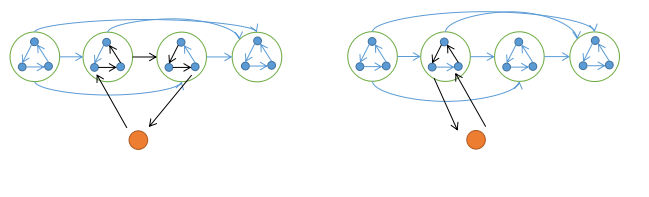
\includegraphics[width=15cm]{file//hamiltonian1.png}
				\end{center}
				\subsubsection{性质三}
				竞赛图一定存在一条哈密尔顿路径。
				
				构造方法为,把竞赛图缩成链之后,把每一个强联通分量的哈密尔顿回路找出来,然后断开其中的一条边与链上的其它点相连。
				\begin{center}
					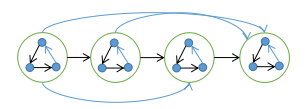
\includegraphics[width=7cm]{file//hamiltonian2.png}
				\end{center}
				\subsubsection{性质四}
				竞赛图中大小为 $n(n\ge3)$ 的强联通分量,大小为 $[3,n]$ 的简单环均存在。
				
				证明。考虑归纳证明,首先 $n=3$ 时显然成立,现在只需证明大小为 $n$ 的强联通分量存在一个大小为 $n-1$ 的简单环。
				
				考虑从联通块中提取出一个点,那么剩下的点缩点一定能形成一条链,并且提取出的这个点一定有一条出边指向链首,一定有一条入边从链尾指向这个点。
				
				当剩下的点形成的为一个联通块时,此时大小为 $n-1$ 的简单环显然成立;当剩下的点形成大于等于 $2$ 个联通块时,可以随意地选择一个联通块中的一个点不走,其它的点构造哈密尔顿路径,最后再通过外面的那个点把首尾相连形成哈密尔顿回路。
				\begin{center}
					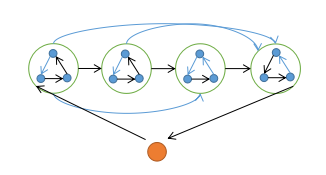
\includegraphics[width=7cm]{file//hamiltonian3.png}
				\end{center}
				\subsubsection{兰道定理}
				竞赛图判定定理。
				
				定义一个竞赛图的比分序列为把竞赛图的每一个点按照出度从小到大排序。一个长度为 $n$ 的比分序列$S_i$ 是合法的当且仅当 $\forall k\in[1,n],\sum_{i=1}^kS_i\ge\binom{n}{k}$ 且当 $k=n$ 时一定取得等号。
		\subsection{二分图与网络流}
			\subsubsection{匹配、边覆盖、独立集与点覆盖}
			\paragraph{定义}
			\begin{itemize}
				\item 匹配:在 $G$ 中没有公共端点的边的集合,记作 $M$
				\item 边覆盖:在 $G$ 中满足任意顶点都至少是集合中一条边的端点的边的集合,记作 $F$
				\item 独立集:在 $G$ 中没有公共边的点的集合,记作 $S$。
				\item 点覆盖:在 $G$ 中任意边都至少有一个端点在集合内的点的集合,同样记作 $S$
			\end{itemize}
			相应的就有:最大匹配,最小边覆盖,最大独立集和最小点覆盖。
			\paragraph{最大匹配与最小边覆盖} 对于无向连通图,最大匹配+最小边覆盖=顶点数
			
			证明:设最大匹配为 $M$ ,最小边覆盖为 $F$ ,则最大匹配中所有的边共覆盖了 $2|M|$ 个顶点,剩下 $|V|-2|M|$ 个节点未覆盖。
			
			考虑在最大匹配的边集中加入一条边,它最多只能多覆盖一个点,因为如果能覆盖两个点的的话它一定就已经在最大匹配中了。由于是要最小边覆盖,那么每次一定是选取一个能覆盖一个点的边加入。
			
			那么就有等式 $|V|-2|M|+|M|=|F|$ ,即 $|M|+|F|=|V|$
			
			\paragraph{最大独立集与最小点覆盖} 对于无向图,最大独立集+最小点覆盖=顶点数
			
			证明:对于任意一个独立集 $S$ ,设它的补集为 $S'$ ,则根据独立集的定义, $S$ 之间一定两两无边,所以任意边的端点一定有一个在 $S'$ 内,所以 $S'$ 为一个点覆盖。
			
			又因为补集有 $|S|+|S'|=|V|$ ,所以有 最大独立集+最小点覆盖=顶点数
			
			\subsubsection{$König$ 定理}
			\paragraph{内容} 在二分图中,最大匹配数=最小点覆盖
			
			首先给出构造方法。设最大匹配为 $M$ 对于二分图最大匹配的求解,是基于增广路定理的。那么当满足最大匹配的时候,从左边任意未匹配点出发,寻找增广路,一定不能满足按照非匹配边-匹配边-非匹配边这样走到一个非匹配点,不然匹配数还可以增加,与最大匹配矛盾。那么从左边所有未匹配点出发,寻找残缺的最短路,标记出所有经过的点。最后左侧未标记的点与右侧被标记的点组成的点集即为一个合法的最小点覆盖。
			
			要证明上述构造正确,只需证明两个事实:构造出的点集大小等于 $|M|$;构造出的是最小点覆盖。
			
			对于第一点,原因是该点集中的任意一个点一定与 $M$ 中的匹配边一一对应。对于左边,如果某个点原本不在最大匹配中,那么它就会被标记;对于右边,如果某个点原本不在最大匹配中,那么它一定不会被标记,因为如果能够通过左边走到它,就形成了一条完整的增广路,与最大匹配定义不符;同时,对于一条匹配边,如果其右边是标记了的,那么一定会标记其左边。所以综上,左边未标记的点与右边标记的点组成的点集一定与匹配边一一对应。
			
			对于第二点,根据匹配的定义,可知覆盖这 $|M|$ 条边至少需要 $|M|$ 个点,所以这已经达到了最小点覆盖的理论下界。
			
			\subsubsection{$Hall$定理}
			\paragraph{内容} 对于二分图,$G=\{V1,V2,E\}$ ,其存在完全匹配当且仅当对于任意属于 $V1$ 的 $k$ 个点,至少与 $V2$ 中 $k$ 个点是相邻的。
			
			\paragraph{必要性} 假设一个图存在完全匹配但不满足 $Hall$ 定理,那么对于左边任意 $K$ 个点,它们连向的点少于 $K$ 个,显然与完全匹配矛盾。
			
			\paragraph{充分性} 假设一个图满足 $Hall$ 定理但不存在完全匹配。首先得到其最大匹配,由于不存在完美匹配,至少可以找到一个未匹配的点。由 $Hall$ 定理,一定能从这个点找到另一个点。如果这另一个点是未匹配点,则与最大匹配定义矛盾;反之如果是匹配点,那么就可以找到它的匹配点,由 $Hall$ 定理,一定又能找到另外一个点,这样一路寻找下去,一定能找出一条增广路,由于最大匹配的定义矛盾了。
				
			\subsubsection{二分图最大匹配}
			\paragraph{Hungary算法} 求解二分图的最大匹配,基于增广路定理,每次寻找一条增广路,将增广路上的匹配边和非匹配边翻转,可以使最大匹配数 $+1$
			\cpp{code//Graph//hungary.cpp}
			\paragraph{Hopcroft-Karp 算法} 依然是基于增广路定理,本质上是 Hungary 算法的优化。在寻找增广路径时,从所有未匹配的左端点出发,寻找多条不相交的增广路径,形成极大增广路径集,然后对增广路径集进行增广。可以认为是把相同长度的增广路径一起增广,且长度随着阶段递增。
			\subsubsection{二分图最大/最小权匹配}
			带权二分图的权值最大的完备匹配称为二分图的最大权匹配。一个比较优秀的算法是 $KM$ 算法,下面均以最大权匹配为例。
			
			$KM$ 算法引入了顶标和相等子图的概念。对于左右两边的顶点分别维护顶标,而只有满足 \texttt{dx[u]+dy[v]=dist} 的边才在相等子图中,每次在相等子图中寻找增广路。如果能够寻找到增广路,则说明找到了最大权匹配;否则,需要修改顶标,扩大相等子图,继续寻找。
			
			关键操作在于顶标的修改。初始的时候,左侧顶标为其连出去的最大边权,而右侧顶标为 $0$ 。当增广失败时,可以得到若干从左边出发,经过非匹配边-匹配边-非匹配边-匹配边 最后回到左边的残缺增广路,称之为交错树。对在交错树中的左顶标减去一个权值 $d$ ,而对在交错树中的右顶标加上一个权值 $d$ 。考虑这样对相等子图的影响,对于一条边:
			\begin{itemize}
				\item 两端都在交错树中,此时依然在相等子图中。
				\item 两端都不在交错树中,此时依然不在相等子图中。
				\item 左端点不在交错树中,右端点在交错树中,顶标和会增大,原来不属于相等子图,现在也不属于。
				\item 左端点在交错树中,右端点不在交错树中,顶标和会减小,可能进入相等子图。
			\end{itemize}
		
			由于目的是扩大相等子图,所以至少要使得一条原来不在相等子图中的边加入相等子图。又因为是要求最大权匹配,所以这个 $d$ 应该是不在相等子图中的边的标号和与边权差值的最小值。用一个 $slack$ 数组记录对于右边所有点的这个最小权,当匹配失败的时候用其中的最小值扩张相等子图。
			\cpp{code//Graph//km.cpp}
			\subsubsection{最大流/最小割}
			求解源汇之间的最大流量,同时也是分割源汇的最小割。
			\paragraph{Edmond-Karp算法} 最基本的增广算法,每次直接 $dfs$ 寻找一条增广路。
			\paragraph{Dinic 算法} 引入分层图优化,每次只在相邻层之间转移,当当前分层的流全部用光时,重构分层图。本质是按照距离从小到大增广。常见优化是当前弧优化。
			\cpp{code//Graph//dinic.cpp}
			\paragraph{ISAP} 同样是引入分层图,不过是从汇点到源点的分层图。每次在找不到增广路时不再重构分层图,而是直接推进标号。常见优化有当前弧优化和 $gap$ 优化。
			\cpp{code//Graph//isap.cpp}
			\subsubsection{费用流}
			即把增广过程用最短路代替。
			\paragraph{消圈定理} 在某个流中,如果其残量网络不存在负环,则它一定是当前流量下的最小费用流。
			\paragraph{$zkw$费用流} 类比最大流中的 Dinic ,$zkw$ 费用流建立最短路分层图,每次只转移最短路图上的增广路。相当于是按照距离从小往大增广。
			\subsubsection{无源无汇上下界可行流}
			无源无汇可行流的条件 
			\begin{itemize}
				\item 对于每一条边,流量大于等于下界  
				\item 对于每一个点,$\sum \mbox{入流}=\sum \mbox{出流}$
			\end{itemize} 
			
			可行流算法的核心是将一个不满足流量守恒的初始流调整成满足流量守恒的流。流量守恒,即 每个点的总流入量=总流出量。
			
			如果存在一个可行流,那么一定满足每条边的流量都大于等于流量的下限。因此我们可以令每条边的流量等于流量下限,得到一个初始流,然后建出这个流的残量网络。(即:每条边的流量等于这条边的流量上限与流量下限之差)这个初始流不一定满足流量守恒,因此最终的可行流一定是在这个初始流的基础上增大了一些边的流量使得所有点满足流量守恒。  
			
			因此我们考虑在残量网络上求出一个另不满足流量守恒的附加流,使得这个附加流和我们的初始流合并之后满足流量守恒,即:  
			
			\begin{itemize}
				\item 如果某个点在所有边流量等于下界的初始流中满足流量守恒,那么这个点在附加流中也满足流量守恒,
				\item 如果某个点在初始流中的流入量比流出量多 $x$,那么这个点在附加流中的流出量比流入量多 $x$。  
				\item 如果某个点在初始流中的流入量比流出量少 $x$,那么这个点在附加流中的流出量比流入量少 $x$。
			\end{itemize}
			
			可以认为附加流中一条从  $u$ 到 $v$ 的边上的一个流量代表将原图中 $u$ 到 $v$ 的流量增大 $1$ 。新建超级源点和超级汇点,补充需要的流量。
		
			\subsubsection{有源有汇上下界可行流}
			
			考虑唯一不满足流量守恒的是两个点 $S$ 和 $T$ ,又因为有 $S$ 流出的流量等于 $T$ 流入的流量,所以连接一条边 $T->S$ ,容量为无穷大,转化为无源无汇上下界,求可行流。最后的可行流就是 $T->S$ 的流量。
			
			\subsubsection{有源有汇上下界最大流}
			
			转化为上面可行流的模型求出可行流后,若可行,把 $T->S$ 无穷大的那条边删去,从原来的源点向原来的汇点求最大流,这样可行流+新图最大流即为有源有汇上下界最大流。  
			
			具体实现的时候,可以不用这么麻烦,直接在上一次剩下的图上跑一边 Dinic 原来的源汇点,不需要去掉那条边,最后也不需要加上新的边,因为直接 Dinic 的时候就会把 $T->S$的反向弧也就是 $S->T$ 上的流量算进去的。
			
			\subsubsection{有源有汇上下界最小流}
			
			同样还是利用 $T->S$ 容量无穷的边得到一个可行流,然后去掉附加源点、附加汇点,并去掉新增的那一条边。从原来的汇点开始沿着反向弧增广求最大流。因为反向跑等于退流,反向弧的最大流相当于就是去掉尽可能多的自由流量。  
			
			另一个做法,先不添加无穷的边,跑一边最大流 $(S,T)$ 再加上这条最大的边,再跑一边最大流 $(S,T)$ ,如果满流了则有解,否则无解,此时 $T->S$ 边上的就是最小流。这样可以更快地 Dinic,因为两边都是同样的源汇点。
	\newpage
	\section{字符串}
		\subsection{字符串基础}
			\subsubsection{字符串 Hash}
			一种快速判断字符串相等的算法。原理基于生日悖论。
	
			常见 Hash 方法
			\cpp{code//String//hash.cpp}
			扩展应用有树 Hash 和图 Hash 。
			\subsubsection{最小循环表示法}
			把一个字符串的第一个字符不断的丢到后面去,这样可以形成最多 $n$ 个字符串。
			
			定义其中字典序最小的为这个字符串的最小循环表示法。
			
			\paragraph{构造方法} 定义两个指针 $i,j$ ,开始的时候分别在 $1,2$ 两个位置。然后向后扫直到扫到一个不相同的字符,假设当前扫的长度为 $k$ ,如果$S_{i+k} < S_{j+k}$,那么当 $j$ 在 $[j,k]$ 区间内的时候始终是没有 $i$ 优的,那么不如直接把 $j$ 移到 $j+k$ 的后面。复杂度 $O(n)$
			\cpp{code//String//minre.cpp}
			\subsubsection{有限状态自动机}
			定义有限状态自动机是一个五元组 $M=(Q, \Sigma, \delta, q0, F)$
			
			\begin{itemize}
				\item Q,状态的非空有穷集合。$\forall q \in Q$,q称为M的一个状态。
				\item $\Sigma$,字符集
				\item $\delta$,转移函数
				\item q0,起始状态,对于字符串而言,一般代表空字符串
				\item F,终止状态集合
			\end{itemize}
			
			\subsubsection{序列自动机}
			能够识别一个序列的所有子序列,用字符串的语言来讲就是能够识别某一个字符串的所有可以子序列(可以不连续)。
			
			其实实现方式就是对每一个位置开一个大小为字符集的链表数组,表示在当前位置后面接上某个字符会转移到哪里。
			\cpp{code//String//seqauto.cpp}
			\subsubsection{Trie树}
			把字符串按照前缀压缩存储的数据结构。
	
			也常用于二进制位的处理。
		\subsection{前缀字符串算法和数据结构}
			\subsubsection{KMP}
			前缀匹配算法,预处理 next 数组优化转移。
			\cpp{code//String//kmp.cpp}
			实时维护 KMP 自动机可以支持可持久化。
			\subsubsection{Aho Corasick自动机}
			KMP 上 Trie 树,支持多串匹配。重要性质在于 $fail$ 树上的祖先关系就是前缀关系。
			\cpp{code//String//aho.cpp}
			\paragraph{Trie 图} 当字符集大小不变时,可以考虑把 AC 自动机补全成 Trie 图减小常数。
		\subsection{回文字符串算法和数据结构}
			\subsubsection{Manacher 算法}
			预处理出以每一个位置为中心的回文半径。
			
			一个小技巧是在每两个字符之间补充一个无关字符,以避免奇数回文和偶数回文的讨论。
			\cpp{code//String//manacher.cpp}
			\subsubsection{回文树/回文自动机}
			建立关于最长回文后缀的数据结构。
			
			原理是一个串本质不同的回文子串只有 $O(n)$ 个,并且在串的后面增加一个字符,最多只增加一个本质不同的回文子串。
			
			回文自动机的每一个节点对应原串的一个本质不同的回文子串,其 $fail$ 指针则是指向它的最长回文后缀。
			
			由于回文有奇数回文和偶数回文两种,所以有两个根。
			
			增量构造即是不断跳 $fail$ 树寻找合法的最长回文后缀。
			\cpp{code//String//pam.cpp}
			由于回文的对称性,回文自动机同时支持从串的两边增量构造。同时维护两个 $last$ 标记就可以了,但需要注意的是,当整个串为一回文串时,需要把两个标记合并。
			\paragraph{一些性质}
			\begin{itemize}
				\item 回文自动机的节点个数 $-2$ 就是本质不同的回文子串个数。(因为要减去两个根节点)
				\item 回文自动机上,节点在 $fail$ 树上的深度就是这个节点对应的字符串的回文后缀的数量。(注意深度不能算两个根)
				\item 一个串的长度超过一半的回文后缀的长度形成一个等差数列。也就是说,一个串的所有回文后缀的长度能够形成不超过 $\log$ 个等差数列。
			\end{itemize}
		\subsection{后缀字符串算法和数据结构}
			\subsubsection{后缀数组}
			把字符串的所有后缀按照字典序排序的算法即后缀排序。
			
			一般采用倍增的方式实现。
			
			维护一个 $Height$ 表示排序后相邻两个子串的最长公共前缀长度,可以结合其它算法支持字符串的信息查询。
			\cpp{code//String//sa.cpp}
			\subsubsection{后缀自动机}
			接收一个字符串所有后缀的自动机,也就是说能够接收所有子串。
			\paragraph{定义}
			\begin{itemize}
				\item $endpos(s)$,是一个集合,对于子串 $s$,它的所有出现过的位置记为 $endpos(s)$ 。如果两个子串的 $endpos$ 集合相等,则把这两个子串归为一类,即在后缀自动机上表示为一个节点。  
				\item  $substring(st)$ ,状态 $st$ 的所有包含的子串集合。
				\item  $shortest(st)$ ,对于状态 $st$ ,其能代表的最短子串。  
				\item  $longest(st)$ ,对于状态 $st$ ,其能代表的最长子串。  
				\item  $parent$ ,对于状态 $st$ , $shortest(st)$ 的任意一个非自己的后缀一定出现在了更多的位置,其中最长的那个,会出现在 $parent(st)$ 的 $endpos$ 中,并且一定是其 $longest$ 。
				\item  $trans(s,c)$ ,表示从 $s$ 这个自动机节点表示的所有字符串后面增加一个字符 $c$ 到达的自动机节点。
			\end{itemize}
			\paragraph{性质}
			\begin{itemize}
				\item 对于 $S$ 的两个子串 $s1,s2$ ,假设有$length(s1) \le length(s2)$,则 $s1$是 $s2$ 的后缀当且仅当$endpos(s2) \subseteq endpos(s1)$。$s1$ 不是 $s2$ 的后缀当且仅当$endpos(s1) \cap endpos(s2)= \emptyset$。
				\item 对于状态 $st$ ,任意$s \in substring(st)$,都有 $s$ 是 $longest(st)$ 的后缀。
				\item 对于状态 $st$ ,任意 $longest(st)$ 的后缀 $s$ ,若$length(shotest(st)) \le length(s) \le length(longest(st))$,那么$s \in substring(st)$
				\item  $substring(st)$ 包含的是状态 $longest(st)$ 的一系列长度连续的后缀。
				\item  $longest(parent(st))$ 一定是 $shortest(st)$ 的最长的后缀,也就是去掉第一个字符的子串。
				\item  $length(shortest(st))=length(longest(parent(st)))+1$
				\item 若 $tranc(st,c)=NULL$,则 $trans(parent(st),c)=NULL$
				\item  $endpos(parent(st))$ 包含了它的所有儿子的 $endpos$,所以 $endpos(parent)$ 可以看作是它的儿子 $endpos$ 的并集。
			\end{itemize}
			\paragraph{构建} 考虑增量构造。记当前已经得到的自动机中末尾字符串代表的节点为 $s$ ,新加的字符是 $c$ 。那么我们可以知道,每增加一个字符,首先肯定要增加一个状态表示 $s+c$ ,然后我们要跳 $s$ 的 $parent$ 树去修改一路上的 $trans$ ,也可能是增加。分三种情况讨论。
			\begin{itemize}
				\item 对于从 $s$ 到根的 $parent$ 树上的路径,如果都没有 $c$ 的转移,那么对这些状态加上 $c$ 的转移就好。最后把新状态的 $parent$ 指向根。
				\item 如果原来 $c$ 的转移 $trans(p,c)$ 这个点的 $longest$ 恰好等于 $p$ 的 $longest+1$,这意味着 $trans(p,c)$ 这个状态只表示了一个 $endpos$ 的集合,也就意味着 $trans(p,c)$ 能够表示的所有串加上一个字符 $c$ 后出现的位置并没有变化。那么此时,我们再增加一个 $c$ 的转移,同样也不会有变化,可以认为只是又增加了一个可行的结束位置。那么直接把新状态的 $parent$ 指向 $trans(p,c)$
				\item $trans(p,c)$ 这个点的 $longest$ 大于 $p$ 的 $longest+1$, 这意味着原来 $trans(p,c)$ 这个自动机节点就表示的是多个字符串的状态,那么此时在 $p$ 后面再增加一个字符 $c$ ,势必与原来的 $trans(p,c)$ 代表的字符串的 $endpos$ 会不一样。那么此时我们就要从原来的 $trans(p,c)$ 这个点拆分出一个点来表示新的 $endpos$ 集合,把原来 $trans(p,c)$ 表示的字符串中长度小于等于 $longest(s)+1$ 的串分裂出去,其它的保留。分裂出去是因为从现在开始,原来这些字符串的 $endpos$ 集合发生了改变。再构造新的 $parent$ 使之指向分裂出去的新点。由于要修改所有长度小于等于 $longest(s)+1$ 的点,那么还要跳 $p$ 的 $parent$ 树修改所有的 $trans(p,c)$ 。
			\end{itemize}
			\cpp{code//String//sam.cpp}
			\subsubsection{广义后缀自动机}
			相比后缀自动机是接收一个串的子串,广义后缀自动机是接收若干串的子串。
	
			只是在插入一个串之后重新从根开始插入即可,注意如果某一个点已经建立了就不用再新建点了。
			\cpp{code//String//lsam.cpp}
\section{计算几何}
	\subsection{直线的表示方法}
	最简单的是用一般式来表示,即 \texttt{Ax+By+c=0} 。  
	
	比较通用的形式是用向量来表示,有两种表示方法,一种是直接用两个不同的点来代表直线;另一种是指定直线上的一个点,然后用一个向量表示其指向方向,方便起见,指定的点通常是与 \texttt{y} 轴的交点。
	\subsection{求三角形面积}
	
	一种比较简介的方法是利用海伦公式 $S=\sqrt{p(p-a)(p-b)(p-c)}$ ,其中 $p=\frac{a+b+c}{2}$
	
	另一种方法是用向量,注意求出的是带符号的面积,所以有的时候也可以用来判断两个向量的相对位置关系。
	
\begin{minted}[bgcolor=bg]{c++}
ld Cross(Point A,Point B){
    return A.x*B.y-A.y*B.x;
}
\end{minted}
	
	\subsection{向量的旋转}
	对于向量 \texttt{(x,y)} 旋转 $\theta$ 后的向量为 $(x\cos\theta-y\sin\theta,x\sin\theta+y\cos\theta)$
	
	\subsection{求直线的交点}
	直接的方法就是带入两条直线的一般式解方程。需要讨论一些情况。  
	
	一种比较简单的写法是用向量加面积的比来求。
	  
	用直线上一个点+指向方向的向量这种方式表示两条直线,如图所示 \texttt{AE} 和 \texttt{BD} ,交点为 \texttt{P} , \texttt{OA} 和 \texttt{OB} 分别为两点的位置向量, \texttt{AE} 和 \texttt{BD} 分别为方向向量,而 \texttt{AA'} 由 \texttt{BD} 平移得到。
	
	\begin{center}
		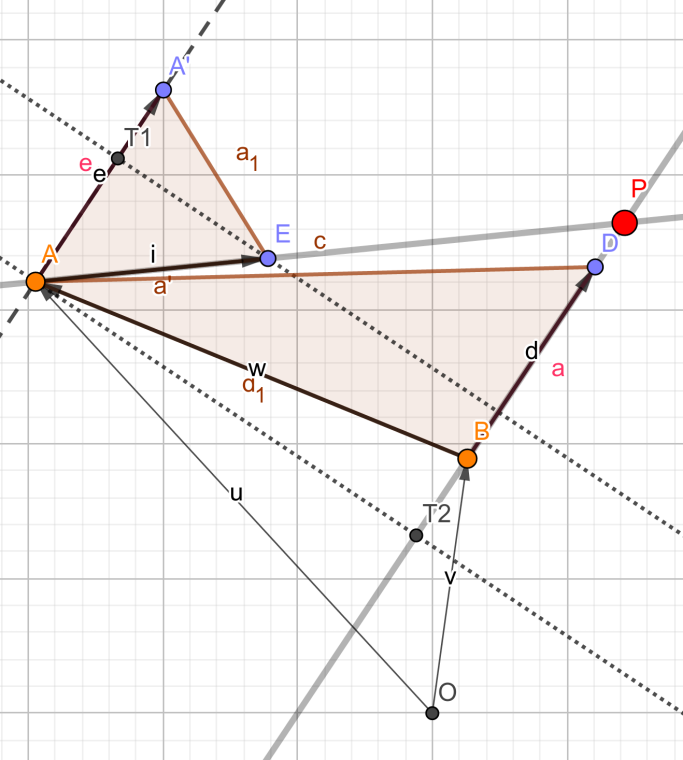
\includegraphics[width=7cm]{file//point.png}
	\end{center}

	能够通过 \texttt{cross} 快速算出两个黄色三角形的面积,然后两个面积之比就是 \texttt{AE} 与 \texttt{AP} 之比,这个由相似三角形可以证明,那么就用 \texttt{A} 点的位置向量加上方向向量的若干倍,得到的就是交点 \texttt{P} 的坐标了。
\begin{minted}[bgcolor=bg]{c++}
Point GetP(Line A,Line B){//.p 为位置向量, .d 为方向向量
    Point dx=A.p-B.p;
    ld t=Cross(B.d,dx)/Cross(A.d,B.d);
    return A.p+A.d*t;
}
\end{minted}
	
	\subsection{半平面交}
	若干个半平面的交集称之为半平面交,通常用来求解二元不等式的相关问题。  
	
	默认半平面为有向向量的左半部分。
	
	一般解法为,先把所有向量按照极角排序,然后考虑增量构造。维护两个双端队列,一个用来维护当前在半平面交上的向量,另一个用来维护在半平面交上相邻向量的交点坐标。加入一个新的向量的时候,判断最后的交点是否在当前向量的左边,如果是,说明前面的向量合法,否则说明前面的某个向量已经被覆盖,需要弹掉。需要用双端队列的原因是,后面向量可能会绕一圈绕回来,把前面的交点弹掉,同样是判断交点是否在当前向量的左边。  
	
	但这样的话,会导致最后面有部分多余的向量,需要再假装把第一个向量再加入,弹掉后面那些交点在右边的向量。  
	
	当向量个数大于等于 \texttt{3} 个,则说明存在解。
	
	需要注意的是,因为半平面交的解有可能是外围的无限大平面,所以一般的做法是在外围加入一个非常大的平行四边形或矩形,把整个半平面限制在这个矩形内。
	
\begin{minted}[bgcolor=bg]{c++}
bool Isleft(Line A,Point B){
    return Cross(A.d,B-A.p)>0;
}
bool check(){
    int L=1,R=1;Q1[1]=A[1];
    for (int i=2;i<=scnt;i++){
        while ((L<R)&&(!Isleft(A[i],Q2[R-1]))) R--;
        while ((L<R)&&(!Isleft(A[i],Q2[L]))) L++;
        Q1[++R]=A[i];
        if (fabs(Cross(Q1[R].d,Q1[R-1].d))<1e-15){
            --R;
            if (Isleft(Q1[R],A[i].p)) Q1[R]=A[i];
        }
        if (L<R) Q2[R-1]=GetP(Q1[R-1],Q1[R]);
    }
    while ((L<R)&&(!Isleft(Q1[L],Q2[R-1]))) R--;
    return R-L>1;
}
\end{minted}
\section{博弈论}
	\subsection{基本定义和性质}
	\subsubsection{必胜点和必败点}
	
	\texttt{P} 必败点,当前先手无论如何必败的点  
	
	\texttt{N} 必胜点,当前先手如果正确操作能够胜利的点
	
	\begin{itemize}
		\item 所有游戏的终止位置都是都是 \texttt{P}   
		\item 任何必胜点一定能进入一个必败点  
		\item 任何必败点只能进入必胜点
	\end{itemize}
	
	\subsubsection{无偏博弈}
	
	无偏博弈是一类任意局势对于游戏双方都是平等的回合制双人游戏。平等的含义是当前的所有可行的走法仅仅只依赖与当前的局势,而与当前谁移动无关。换而言之,两个人除了先后手的区别之外就不存在任何区别。除此之外,还需要满足一下性质:  
	
	\begin{itemize}
		\item 完全信息,任何一个游戏者都能够知晓整个游戏状态。  
		\item 无随机行动,所有的行动都会转移到一个唯一确定的状态。  
		\item 有限步内游戏会终止,此时有唯一的胜者。
	\end{itemize}
	
	\subsection{正确性的证明方法}
	
	根据定义,证明一种判断 \texttt{position} 的性质的方法的正确性,只需证明三个命题
	
	\begin{itemize}
		\item 这个判断将所有结束位置判断为 \texttt{P} 点
		\item 根据这个判断得出的 \texttt{N} 点一定能走到一个 \texttt{P} 点
		\item 根据这个判断得出的 \texttt{P} 点一定不能走到一个 \texttt{P} 点
	\end{itemize}
	\subsection{对抗搜索}
	一般而言,站在两个人的立场上进行搜索。
	
	通常为了方便处理,将一个人的权值设置为负数,另一个为正数,这样就可以在不同的层进行 \texttt{min-max} 搜索。
	
	\paragraph{\texttt{Alpha-Beta}剪枝} \texttt{Alpha-Beta} 剪枝在于把父亲或者祖先的信息向下传递,若发现当前的答案无论如何都无法更新祖先时,直接返回。
	\paragraph{记忆化}对于可记忆的搜索,可以加上记忆化或转化为可以记忆化的方式,通常是对于某一局面,两人不论谁先操作,得到的结果一样时,可以记忆化。
	\subsection{常见模型}
	
	\subsubsection{巴什博弈\texttt{(Bash Game)}}
	\paragraph{基本问题} 给出一堆 \texttt{n} 个石子,每次可以选择 \texttt{1-m} 个,最后无法选择的人输,求先后手的获胜情况。
	\paragraph{结论} 当 \texttt{(m+1)|n} 的时候,先手必败,否则先手必胜。
	\paragraph{证明} 可以知道,\texttt{[1,m]} 内是先手必胜的,\texttt{m+1} 只能转移到 \texttt{N} 节点,所以是 \texttt{P} 节点,依次类推
	
	一般而言,都是用这种分析必胜、必败区间的方法来证明或者归纳其正确性。
	
	\subsubsection{尼姆博弈\texttt{(Nim Game)}}
	\paragraph{基本问题} 给出若干堆石子,每次可以从某堆石子中任意选取若干个,不能操作者输。
	\paragraph{结论} 当所有堆石子异或和为 \texttt{0} 的时候,先手必败,否则先手必胜
	\paragraph{证明} 可以直接用 \texttt{SG} 定理来证,也可以根据必胜必败点的定义来证。下面证明定义的三个命题成立。
	
	\begin{itemize}
		\item 命题一:终止位置只有一个,那就是所有石子堆都为 \texttt{0} ,此时异或和为 \texttt{0} ,得证  
		\item 命题二:任意一个非 \texttt{0} 的异或组合一定能找到那个最高位 \texttt{1} 的来源使之走到一个异或和为 \texttt{0} 的组合,得证  
		\item 命题三:任意一个异或和为 \texttt{0} 的组合去掉任意一个数后异或和都不为 \texttt{0} ,得证  
	\end{itemize}
	三个命题均成立,所以成立。
	
	\paragraph{尼姆博弈的扩展形式}
	\begin{itemize}
		\item 限定每次取的上限,即每次只能取 \texttt{[1,m]} 个
	
		相当于与 \texttt{Bash Game} 进行组合,那么将所有石子对 \texttt{(m+1)} 取模再进行 \texttt{Nim} 游戏
	
		\item 允许从 \texttt{K} 堆石子中取
	
		一般在一堆中取是作异或,而异或就是二进制不进位加法。那么从 \texttt{K} 堆中取就是对所有石子的二进制位作 \texttt{K+1} 进制的不进位加法
	
		\item 阶梯博弈,每一次将一堆石子的一部分从当前阶移动到下一阶,不能移动者输
	
		只需要考虑奇数阶的石子的异或和,因为如果是偶数阶的话,对方操作一次偶数阶,可以对应的操作奇数阶使得恢复到原来的状态。
	\end{itemize}
	
	\subsubsection{威佐夫博弈 \texttt{(Wythoff Game)}}
	\paragraph{基本问题} 两堆石子,每次可以在一堆中取,也可以在两堆中同时取相同多个,不能取的人输。
	\paragraph{结论} 先手必败的情况一定满足 $(\lfloor ka\rfloor,\lfloor ka^2 \rfloor )$ ,其中 $a=\frac{\sqrt{5}+1}{2}$
	
	\subsection{\texttt{Sprague-Grundy}定理与\texttt{Sprague-Grundy}函数}
	\subsubsection{定义}
	\paragraph{\texttt{SG}函数} 对于每一个状态的尼姆数的函数称为 \texttt{SG} 函数。
	\paragraph{\texttt{SG}定理} 所有一般胜利下的无偏博弈都能够转化成尼姆数表达的尼姆堆博弈,一个无偏博弈的尼姆值定义为这个博弈的等价尼姆数。
	
	对于当前游戏 \texttt{X},它可以拆分成若干个子游戏$x_1,x_2,x_3,\dots,x_n$。那么$SG(X)=SG(x_1)\oplus SG(x_2)\oplus\dots\oplus SG(x_n)$。定义 \texttt{P} 状态和空集的 \texttt{SG} 函数为 \texttt{0} ,而对于当前状态 \texttt{x} ,它的 \texttt{SG} 值为其所有后继的 \texttt{mex} 。
	
	\subsubsection{\texttt{Anti-SG} 游戏和 \texttt{SJ}定理}
	\paragraph{基本问题}给定 \texttt{n} 堆石子,每次可以从任意一堆石子中取走不少以一个石子,拿到最后一个石子的人输。
	\paragraph{\texttt{SJ}定理} 对于一个\texttt{Anti−SG} 游戏,如果我们规定当前局面中所有单一游戏的 \texttt{SG}为 \texttt{0}时,游戏结束,则先手必胜的条件为:
	\begin{itemize}
		\item 游戏的\texttt{SG}值不为\texttt{0},且存在一个单一游戏的\texttt{SG}值大于\texttt{1}
		\item 游戏的\texttt{SG}值为\texttt{0},且不存在一个单一游戏的\texttt{SG}值大于\texttt{1}。
	\end{itemize}
	
	\subsubsection{\texttt{Multi-SG}游戏}
	\paragraph{基本问题} 给定 \texttt{n} 堆石子,每次可以取走任意数量个,或者将一堆式子拆分成两堆(事实上更多也是可行的)非空石子,不能操作者输,判定胜负。
	\paragraph{结论} 本质还是 \texttt{SG} 定理的运用。对于每个状态的后继状态,既可以是拆分,也可以是数量的减少,对所有后继状态取 \texttt{mex}
	
	当拆分堆数为 \texttt{2} 时,有如下结论。
	\begin{align}
	SG(x)=\begin{cases} x-1&(x\ mod\ 4=0)\\ x&(x\ mod\ 4=1\&2)\\ x+1&(x\ mod\ 4=3) \end{cases}\nonumber		
	\end{align}
	\subsubsection{翻硬币游戏}
	\paragraph{基本问题}有若干枚硬币,每次按照一定的规则翻转硬币,强制要求最右边的一定必须从正面翻到背面。无法操作者输。
	\paragraph{结论}当前局面的 \texttt{SG} 值是所有正面朝上的硬币的 \texttt{SG} 值单独存在时的 \texttt{SG} 函数的异或和。
	\section{其它}
		\subsection{STL}
		\subsubsection{系统堆}
		系统本身有一种已经实现好的堆 \mintinline{c++}{priority_queue} 。但是由于其底层是用 vector 实现的,当不开 O2 的时候常数较大。
		
		但其实 \texttt{STL} 里已经提供了直接操作堆的方法。当堆的大小确定的时候,不妨采用这种实现方式。
		
		\texttt{make\_heap}: 根据指定的迭代器区间以及一个可选的比较函数,来创建一个 \texttt{heap}。 复杂度 $O(n)$
		
		\texttt{push\_heap}: 把指定区间的最后一个元素插入到 \texttt{heap}中。复杂度 $O(\log n)$
		
		\texttt{pop\_heap}: 弹出 \texttt{heap} 顶元素, 将其放置于区间末尾。复杂度 $O(\log n)$
		
		\begin{minted}[bgcolor=bg]{c++}
		class heap{
		public:
		state H[maxH];int c;
		void push(state x){
		H[++c]=x;push_heap(&H[1],&H[c+1]);
		}
		state top(){
		return H[1];
		}
		void pop(){
		pop_heap(&H[1],&H[c+1]);--c;
		}
		bool empty(){
		return c==0;
		}
		};
		\end{minted}
		\subsection{分块}
类似线段树,但是分块对标记的性质要求更一般化了。

通常的做法是对每一个块维护一个标记,当是对块进行整体操作的时候,直接打标记,否则暴力重构块。
\subsubsection{莫队算法}
基于分块的离线算法。

基本内容是将左区间按照所在块编号排序,当在同一区间的时候,按右端点排序。

这样一来,当在同一个块内移动的时候,左端点移动的距离是 $O(\sqrt{n})$ 右端点是 $O(n)$ ,而总共左区间的变化只会有 $O(\sqrt{n})$ 次,所以总复杂度就是 $O(n \times \sqrt{n})$

只要求信息支持能从当前维护的区间单点增量即可。

\subsubsection{带修莫队}
带修莫队,其实就是在原来对序列分块的基础上再增加一维对时间的分块。排序的时候先按时间,再按序列位置;增量的时候,同时要维护一个当前时间戳。

\subsubsection{树上分块}
如果采用序列分块的方式直接映射到到树上分块,会有序列中相邻元素在树上相距很远的问题。单独以子树或者儿子作为分块参考又会导致分块的不均匀,所以一般的分块方式是参考 \texttt{[SCOI2005]王室联邦}。

具体操作是,维护一个与 \texttt{dfs} 相关的栈,每次进入一个子树的时候,先记录下栈顶,然后依次递归整个子树。当当前栈顶与之前记录下的栈顶之间的元素超过划定的块大小时,把这其中的元素划分到一个新块。当整棵子树完成时,把当前点加入栈中。最后要处理一些多余的点,把这些分到最后的块中即可。
\begin{minted}[bgcolor=bg]{c++}
void dfs(int u,int fa){
int nowtop=top;
for (int i=Head[u];i!=-1;i=Next[i])
if (V[i]!=fa){
dfs(V[i],u);
if (top-nowtop>=blocksize)
{
blockcnt++;
while (top!=nowtop) Belong[St[top--]]=blockcnt;
}
}
St[++top]=u;return;
}
\end{minted}

\subsubsection{树上莫队}
如果是查询树上子树信息,则转成对树的 \texttt{dfn} 序作序列莫队,或者 \texttt{dsu on tree}。

否则,则是查询路径信息。进行树上分块,然后同样的维护当前某个路径 \texttt{(u,v)} 的两个端点及答案。移动的时候,分别对两条路径上的点翻转。正确性的证明方法,就是从当前路径移动到另一条路径,直接对两组端点直接的路径取树上路径异或。为了方便处理,通常不把 \texttt{lca} 记录在这个答案中,只在每次算答案的时候临时地把 \texttt{lca} 加入。

\begin{minted}[bgcolor=bg]{c++}
void Move(int u,int v)
{
int lca=LCA(u,v);
while (u!=lca) Reverse(u),u=Fa[0][u];
while (v!=lca) Reverse(v),v=Fa[0][v];
return;
}
\end{minted}
\texttt{Reverse} 即点翻转,原来在路径上的现在从路径中去掉,反之加入路径。

\subsection{\texttt{Meet in the middle}}
对于一些集合的查询问题,可以把集合分成两个部分,分别求信息,然后枚举组合一下。

\subsection{状态压缩}
把与决策相关的信息通过压缩的方式压起来。常见的有二进制压位、整数拆分压位和最小表示法。

\subsection{斜率优化}
常见于将二维的 \texttt{DP} 优化到一维。

一般的推导方式是,讨论前面到当前的两种转移的优劣,列出不等式得到斜率形式,转变为维护凸包。另外也有半平面交的解释方法。

根据 \texttt{x,y} 两维的单调情况,选择单调栈/单调队列/平衡树来维护凸包,采用暴力弹/二分/二叉树查询的方式来查询答案。

\subsection{决策单调}
类似斜率优化,一般用于维护 \texttt{DP} 。当代价的函数满足比如二次函数这种增长很快的形式时,可以考虑决策单调。有两种形式。
一种是对于当前决策,如果小于另一个决策,并且以后都不可能更优,则直接把这个决策舍弃掉。维护一个类似单调栈的东西,比较两个决策点的时候,二分得到后一个超过前一个的时间,与当前时间比较。

另一种是分治地来做。如果当前点 \texttt{i} 的最优决策点在 \texttt{j} 那么在 \texttt{i} 左边的点的最优决策点不会大于 \texttt{j} ,而在右边的不会小于 \texttt{j} , 那么就可以把询问区间和决策区间从这里分裂开来,分治地求解子问题。

\subsection{摊还分析}
通常用于时间复杂度的分析中,像是 \texttt{KMP},\texttt{AC} 自动机, \texttt{Splay,LCT} 还有一些线段树的复杂度证明需要用到摊还分析。一般来说有两种。

\paragraph{核算法} 每一种操作有一个实际的代价,再对每种操作定义一个或许与实际代价不同的摊还代价。可以认为是一些操作在满足自己的基础上还存放了一些代价供其它操作使用。

\paragraph{势能分析} 与核算法类似,不过是定义一些操作增加势能另一些减少势能。

\subsection{树套树}
把数据结构嵌套使用。常数较大。

\subsection{\texttt{dsu on tree}}
基于重链剖分的离线子树查询方式。

扫描的时候,对于轻儿子,暴力扫描加入答案,并且在计算完后暴力清除,而重儿子保留下来,递归重儿子直接计算。

复杂度证明是基于树上任意一个点到根的路径在重链剖分中只会有 \texttt{log} 个重链,也就是说最多被暴力计算 \texttt{log} 次。

\subsection{平面距离}
\subsubsection{欧几里得距离}
多维空间中两点的直线距离  

$$\sqrt{(x1-x2)^2+(y1-y2)^2+……+(k1-k2)^2}$$

\subsubsection{曼哈顿距离}
两点横纵坐标差的绝对值之和

$$|x1-x2|+|y1-y2|$$

\subsubsection{切比雪夫距离}
坐标差中的较大值
$$max(|x1-x2|,|y1-y2|)$$

\subsubsection{切比雪夫距离与曼哈顿距离的转化}
考虑在二维平面上,与原点曼哈顿距离为$1$的点

\begin{center}
	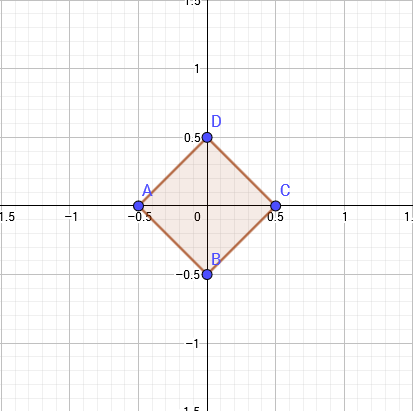
\includegraphics[width=7cm]{file//manhattan.png}
\end{center}

那么,与原点切比雪夫距离为$1$的点为 

\begin{center}
	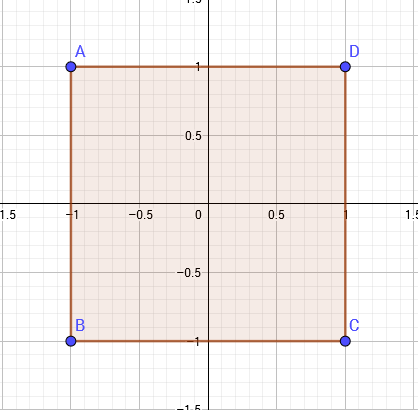
\includegraphics[width=7cm]{file//qiebixuefu.png}
\end{center}

可以发现,第二个图相当于把第一个图旋转$45°$再放大一倍。  

所以曼哈顿距离中的点$(x,y)$转化到切比雪夫中就是$(\frac{x+y}{2},\frac{x-y}{2})$	
\subsection{平面图与对偶图}
对于平面图,可以将其转化为对偶图。具体来说,对于原来的每个平面区域建立一个点,而分割两个平面的边变成连接两个点的边。

有着一些良好的性质,比如平面图的最小割就是对偶图的最短路。
\subsection{二进制分组}
对于维护的信息,从大到小每二进制大小个维护一组。当有两组大小相同时,将两组合并。

本质上是一个动态构建线段树的过程。
	\section{参考资料}
	《Pollard-rho算法简要分析》,ljt12138,http://ljt12138.blog.uoj.ac/blog/3524
	
	《一些特殊的数论函数求和问题》,朱震霆,$2018$国家候选队论文集
	
	《【学习笔记】Min25筛》,cz\_xuyixuan,https://blog.csdn.net/qq\_39972971/article/details/81543972
	
	《炫酷反演魔术》,vfleaking,http://vfleaking.blog.uoj.ac/blog/87
	
	《反演魔术:反演原理及二项式反演》,miskcoo,http://blog.miskcoo.com/2015/12/inversion-magic-binomial-inversion
	
	《竞赛图的一些性质》,zwl,https://www.cnblogs.com/acha/p/9042984.html
	
	《[竞赛图判定定理]兰道定理(Landau's Theorem)介绍及其一种证明》,a\_crazy\_czy,https://blog.csdn.net /a\_crazy\_czy/article/details/73611366
\end{document}
